\documentclass{article}
\usepackage[utf8]{inputenc}
\usepackage{graphicx}
\usepackage{listings}
\usepackage{mathtools}
\usepackage{pdfpages}
\usepackage{verbatim}
\usepackage{geometry}
 \geometry{
 a4paper,
 total={170mm,257mm},
 left=20mm,
 top=20mm,
 }
\usepackage{xcolor}
\usepackage{longtable}
\usepackage{array}
\usepackage{tabularx}
\usepackage{etoolbox} 
\usepackage{lmodern}
\usepackage{refcount}
\usepackage[hidelinks,bookmarks=false,plainpages=false,pdfpagelabels]{hyperref}
\usepackage{subfiles}
\setlength{\emergencystretch}{3em}

% -------- TABLE SETTINGS --------
\renewcommand{\arraystretch}{2.0}
\renewcommand\tabularxcolumn[1]{m{#1}}

% -------- COLUMN TYPES --------
\newcolumntype{C}[1]{>{\centering\arraybackslash}m{#1}} 
\newcolumntype{L}[1]{>{\raggedright\arraybackslash}p{#1}}

% ---------------- LISTINGS SETUP ----------------
\definecolor{codegreen}{rgb}{0,0.6,0}
\definecolor{codegray}{rgb}{0.5,0.5,0.5}
\definecolor{codepurple}{rgb}{0.58,0,0.82}
\definecolor{backcolour}{rgb}{0.95,0.95,0.92}

\lstdefinestyle{mystyle}{
    backgroundcolor=\color{backcolour},    
    commentstyle=\color{codepurple},
    keywordstyle=\color{blue},
    stringstyle=\color{codegreen},
    basicstyle=\ttfamily\footnotesize,
    breakatwhitespace=false,         
    breaklines=true,                 
    captionpos=b,                    
    keepspaces=true,                 
    numbers=left,
    numberstyle=\tiny\color{codegray},
    numbersep=5pt,
    showspaces=false,              
    showstringspaces=false,
    showtabs=false,                  
    tabsize=2,
    frame=single,
    columns=flexible
}
\lstset{style=mystyle}

% -------- FIXED INDEX LOGIC --------
\makeatletter
\newcommand{\MyIndexData}{} 
\newcommand{\indexentryline}[3]{%
    \gappto\MyIndexData{#1 & #2 & #3 & \expagerange{#1} & \\ \hline}
}
\newcommand{\expagerange}[1]{%
    \ifnum#1=19
        77--78%
    \else
        \getpagerefnumber{expstart:#1}--\number\numexpr\getpagerefnumber{expstart:\number\numexpr#1+1\relax}-1\relax
    \fi
}
\newcommand{\experiment}[2]{%
    \clearpage
    \refstepcounter{section}%
    \label{expstart:\thesection}%
    \protected@write\@auxout{}{
        \string\indexentryline{\thesection}{#1}{#2}
    }%
    \addcontentsline{toc}{section}{\protect\numberline{\thesection}#1}%
    \noindent\textbf{\Large Experiment No: \thesection} \hfill {\normalsize Date: #2}
    \section*{#1}
}
\newcommand{\displayindex}{%
    \begin{longtable}{|C{1cm}|L{7.2cm}|C{2.0cm}|C{1.8cm}|C{2.0cm}|}
    \hline
    \textbf{No.} & \textbf{Experiment Name} & \textbf{Date} & \textbf{Page No.} & \textbf{Signature} \\ \hline
    \endhead
    \MyIndexData
    \end{longtable}
}
\makeatother

\begin{document}

% ================= TITLE PAGE 1 =================
\thispagestyle{empty}
\begin{center}
    \Huge{\textbf{COLLEGE OF ENGINEERING\\TRIVANDRUM}}
    \vspace{1cm}
    
    
\includegraphics[scale=0.5]{assets/cet.jpeg}
    
    \huge{DEPARTMENT OF \\ COMPUTER SCIENCE AND ENGINEERING}
    \vspace{1cm}
    
    \hrule
    \vspace{0.8cm}
    \Large{\textbf{CSL 332\\NETWORKING LAB}}
    \vspace{0.8cm}
    \hrule
    
    \vspace{3cm}
    \Huge{Shravan Nander Pandala\\TVE23CS131\\S6 CSE\\(2023-2027 BATCH)}
\end{center}

\newpage

% ================= TITLE PAGE 2 (BONAFIDE) =================
\thispagestyle{empty}
\begin{center}
    \Huge{\textbf{COLLEGE OF ENGINEERING\\TRIVANDRUM}}
    \vspace{1cm}
    
    
\includegraphics[scale=0.5]{assets/cet.jpeg}
    
    \huge{DEPARTMENT OF \\ COMPUTER SCIENCE AND ENGINEERING}
    \vspace{1cm}
    
    \hrule
    \vspace{0.8cm}
    \Large{\textbf{CSL 332\\NETWORKING LAB RECORD}}
    \vspace{0.8cm}
    \hrule
    
    \vspace{3cm}
    \Large{Certified that this is a bonafide record of \textbf{Shravan Nander Pandala, TVE23CS131} of \textbf{S6 CSE}, done as part of Networking Lab during the year 2025-2026.}
    
    \vspace{4cm}
\noindent\normalsize\textbf{FACULTY IN CHARGE \hfill EXTERNAL EXAMINER}
\end{center}

\newpage

% ================= INDEX =================
\pagenumbering{gobble}
\begin{center}
\section*{Index}
\end{center}
\displayindex
\newpage

% ================= TABLE OF CONTENTS =================
\pagenumbering{roman}
\tableofcontents
\newpage
\pagenumbering{arabic}

% ================= EXPERIMENTS =================


\experiment{Familiarization of Linux commands}{19/12/2025}

\subsection{Aim}
To familiarize with Linux networking-related commands.

\subsection{Theory}
The following are some commonly used Linux networking commands and their syntax.

\vspace{0.5cm}

\noindent\textbf{ifconfig}
\begin{itemize}
    \item It stands for interface configurator.
    \item It is used to initialize an interface, configure it with an IP address, and enable or disable it. It is also used to display the route and network interface.
    \item Syntax: \texttt{ifconfig [...OPTIONS] [INTERFACE]}
\end{itemize}
\noindent\textbf{ip}
\begin{itemize}
    \item It is the latest version of ifconfig command and is used to show or manipulate routing and network devices.
    \item Syntax: \texttt{ip [ OPTIONS ] OBJECT COMMAND --help}
\end{itemize}

\noindent\textbf{ping}
\begin{itemize}
    \item It stands for Packet Internet Groper.
    \item It is used to test network connectivity.
    \item It works by sending one or more ICMP (Internet Control Message Protocol) Echo Request packets to a destination IP and waiting for a reply.
    \item Syntax: \texttt{ping [OPTIONS] DESTINATION}
\end{itemize}

\noindent\textbf{traceroute}
\begin{itemize}
    \item It is used to determine the path to a target and the delay in reaching the same.
    \item Syntax: \texttt{traceroute [options] host-address [pathlength]}
\end{itemize}

\noindent\textbf{tracepath}
\begin{itemize}
    \item It is similar to the traceroute command but it does not require root privileges.
    \item Syntax: \texttt{tracepath [-n] [-b] [-l pktlen] [-m max] [-port] destination}
\end{itemize}

\noindent\textbf{netstat}
\begin{itemize}
    \item It stands for network statistics.
    \item It provides statistical figures about different interfaces which include open sockets, routing tables, and connection information.
    \item Syntax: \texttt{netstat [OPTIONS]}
\end{itemize}

\noindent\textbf{ss}
\begin{itemize}
    \item It stands for socket statistics.
    \item It is similar to netstat but it can display more TCP and state information than other tools.
    \item Syntax: \texttt{ss [options]}
\end{itemize}

\noindent\textbf{dig}
\begin{itemize}
    \item It stands for Domain Information Groper.
    \item It is used in DNS lookup to query the DNS name server and to troubleshoot DNS related issues.
    \item It is mainly used to verify DNS mappings, MX Records, host addresses, and all other DNS records for a better understanding of the DNS topography.
    \item Syntax: \texttt{dig [server] [name] [type]}
\end{itemize}

\noindent\textbf{nslookup}
\begin{itemize}
    \item It stands for Name Server Lookup.
    \item It is similar to dig command, used for fetching dns information.
    \item Syntax: \texttt{nslookup [option]}
\end{itemize}

\noindent\textbf{route}
\begin{itemize}
    \item It displays and manipulates the system routing table.
    \item Syntax: \texttt{route [option]}
\end{itemize}

\noindent\textbf{host}
\begin{itemize}
    \item It displays the domain name for a given IP address and the IP address for a given hostname. It can also be used for DNS lookup.
    \item Syntax: \texttt{host [-aCdlriTWV] [-c class] [-N ndots] [-t type] [-W time] [-R number] [-m flag] hostname [server]}
\end{itemize}

\noindent\textbf{arp}
\begin{itemize}
    \item It stands for Address Resolution Protocol.
    \item It is used to view and add content to the kernel's ARP table.
    \item Syntax: \texttt{arp [-v] [-i if] [-H type] -a [hostname]}
\end{itemize}

\noindent\textbf{iwconfig}
\begin{itemize}
    \item It is used to configure the wireless network interface.
    \item Syntax: \texttt{iwconfig [options]}
\end{itemize}

\noindent\textbf{hostname}
\begin{itemize}
    \item It is used to view and set the hostname of the system.
    \item Syntax: \texttt{hostname -v -a --alias -d --domain -f --fqdn -A --all-fqdns -i --ip-address -I --all-ip-addresses --long -s --short -y --yp --nis}
\end{itemize}

\noindent\textbf{curl \& wget}
\begin{itemize}
    \item They are used to download files from the internet through CLI.
    \item Syntax: \texttt{curl -o [url]}, \texttt{wget [url]}
\end{itemize}

\noindent\textbf{tcpdump}
\begin{itemize}
    \item It is used to capture and display the traffic information in a network interface.
    \item Syntax: \texttt{tcpdump [options]}
\end{itemize}

\noindent\textbf{iftop}
\begin{itemize}
    \item It is used to monitor network bandwidth.
    \item Syntax: \texttt{iftop [options]}
\end{itemize}

\noindent\textbf{whois}
\begin{itemize}
    \item It is used to fetch all information related to a website.
    \item Syntax: \texttt{whois [url]}
\end{itemize}

\noindent\textbf{mtr}
\begin{itemize}
    \item It is used to display packet-route information along with per-hop ping time.
    \item Syntax: \texttt{mtr [options]}
\end{itemize}

\noindent\textbf{ethtool}
\begin{itemize}
    \item It is used to configure Ethernet devices on Linux.
    \item Syntax: \texttt{ethtool [options]}
\end{itemize}

\subsection*{Algorithm}
\begin{enumerate}
    \item Open the Linux terminal.
    \item Execute various networking commands to understand their syntax and usage.
    \item Analyze the output for network interface details, connectivity, and DNS resolution.
    \item Capture output screenshots for documentation and label them sequentially.
\end{enumerate}

\subsection{Output}

\begin{center}
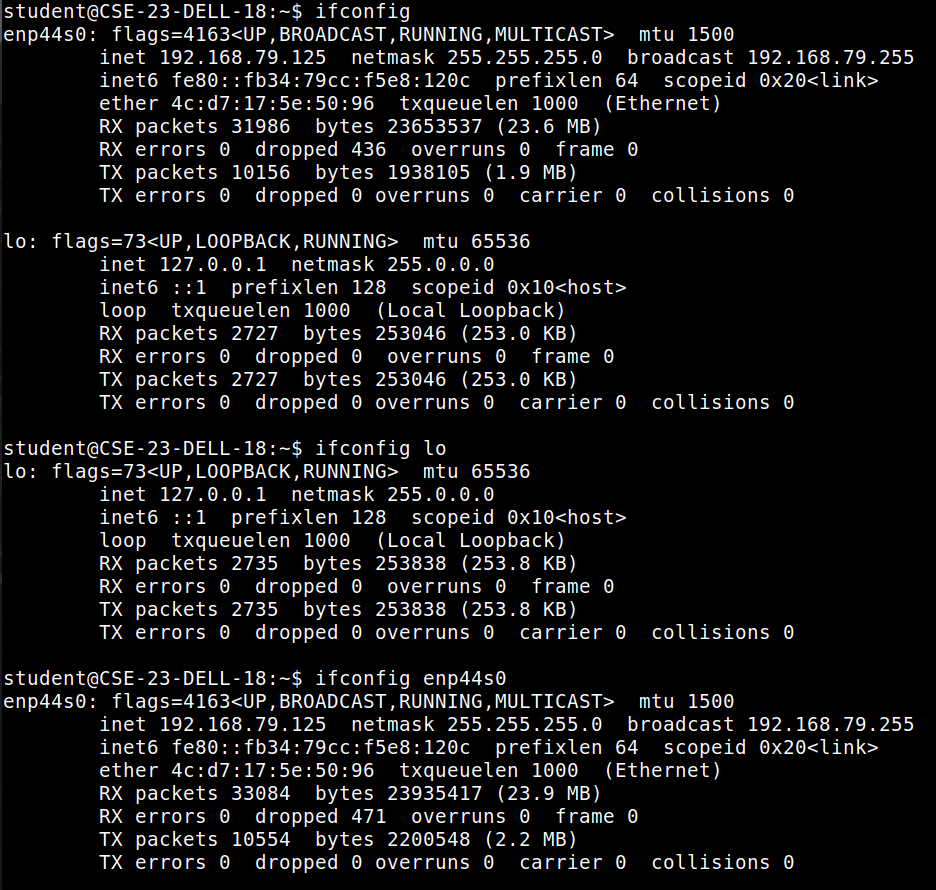
\includegraphics[width=0.90\textwidth]{assets/screenshots/cycle1/ifconfig.png} \\
\textbf{ifconfig} \\[0.35cm]

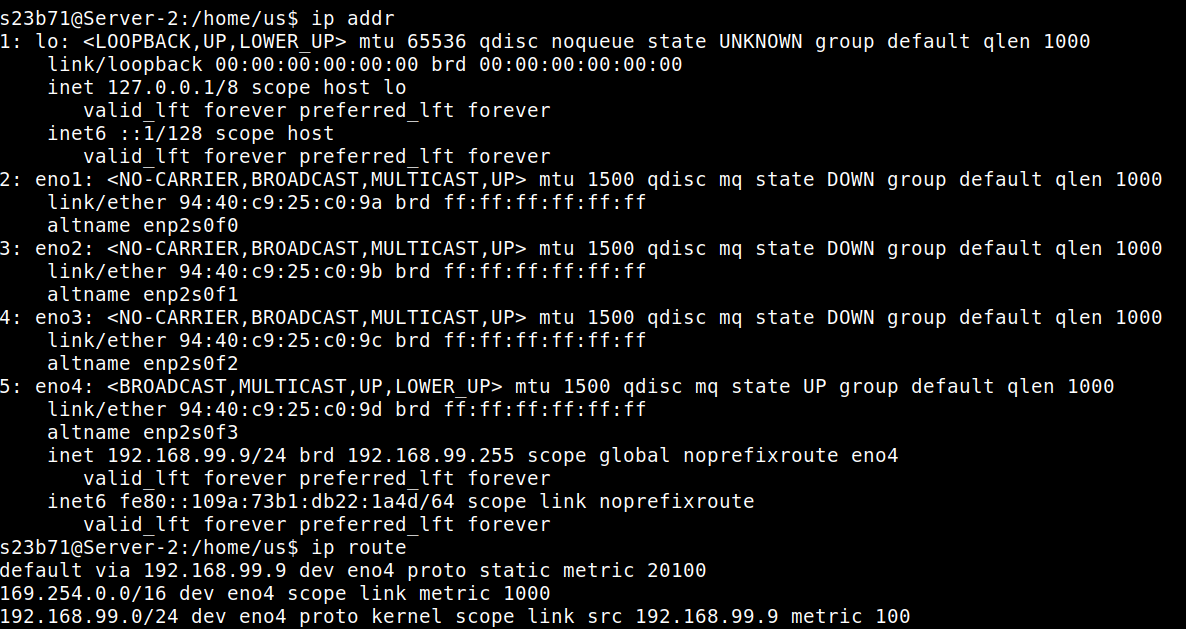
\includegraphics[width=0.90\textwidth]{assets/screenshots/cycle1/ip.png} \\
\textbf{ip addr} \\[0.35cm]

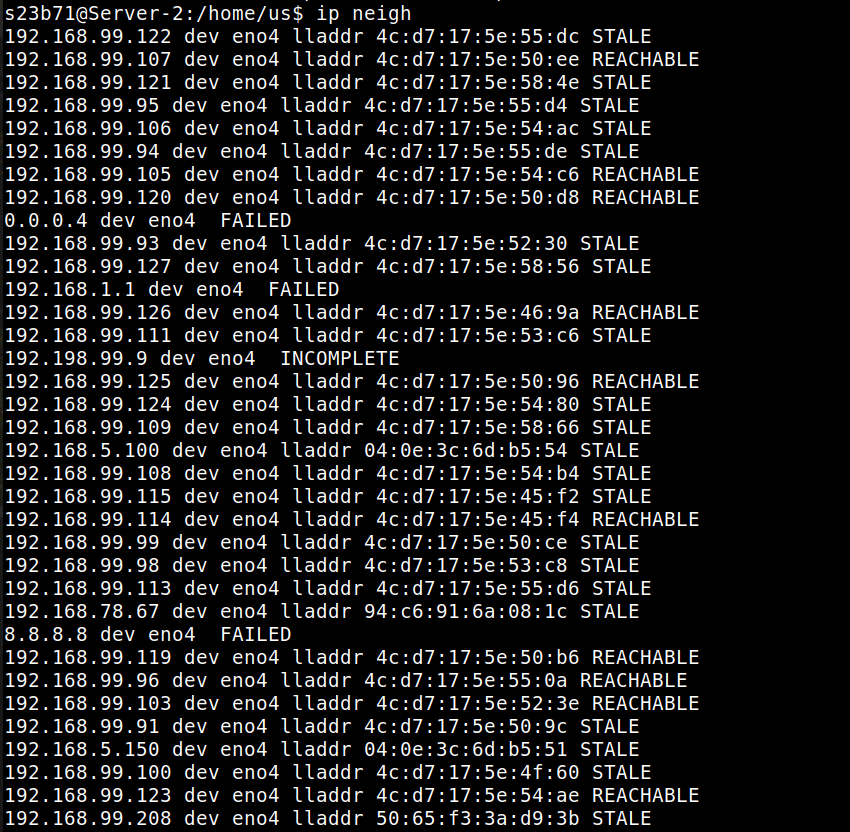
\includegraphics[width=0.90\textwidth]{assets/screenshots/cycle1/ip2.png} \\
\textbf{ip route} \\[0.35cm]

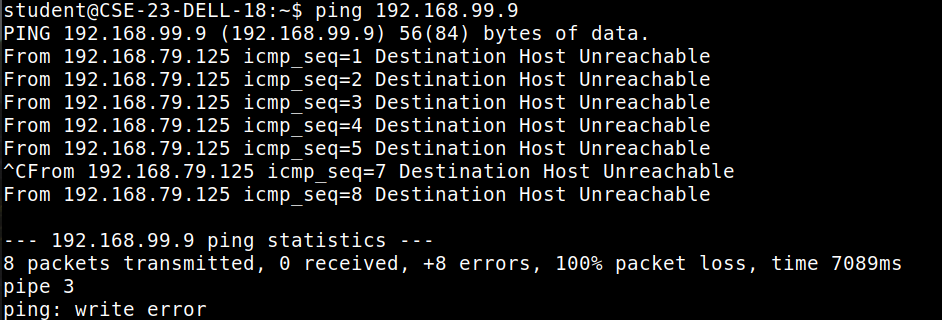
\includegraphics[width=0.90\textwidth]{assets/screenshots/cycle1/ping.png} \\
\textbf{ping} \\[0.35cm]

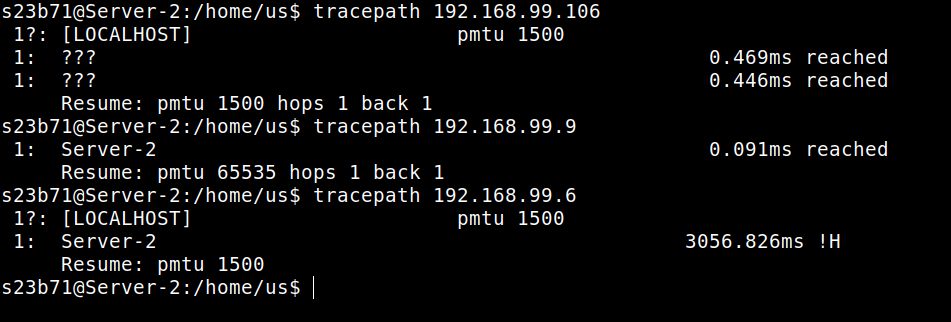
\includegraphics[width=0.90\textwidth]{assets/screenshots/cycle1/tracepath.png} \\
\textbf{tracepath} \\[0.35cm]

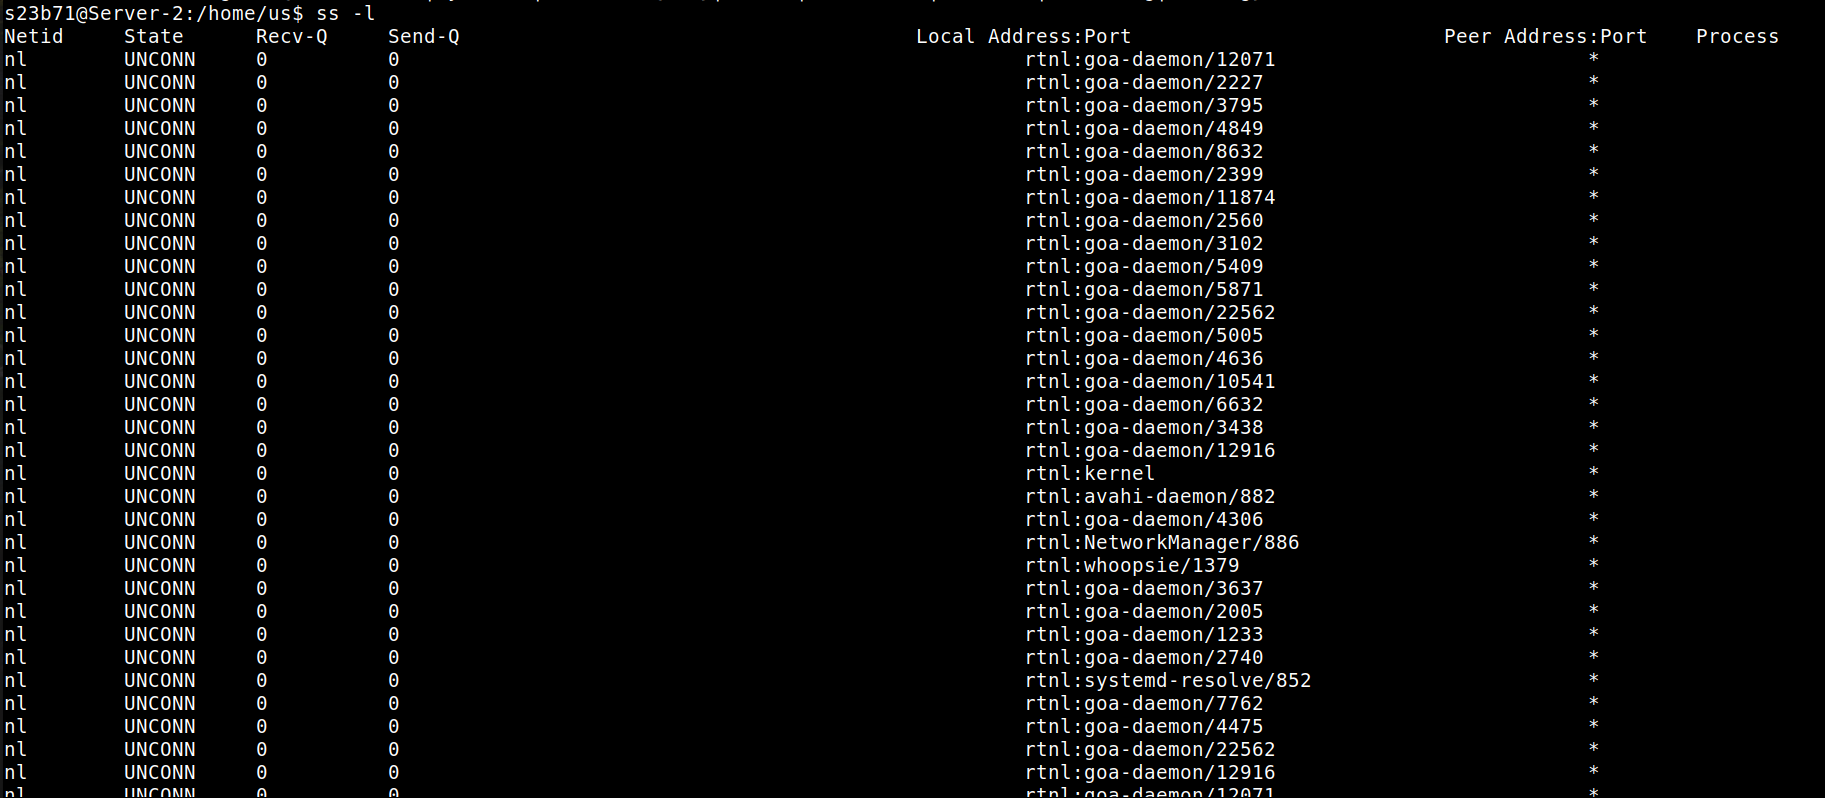
\includegraphics[width=0.90\textwidth]{assets/screenshots/cycle1/ss.png} \\
\textbf{ss} \\[0.35cm]

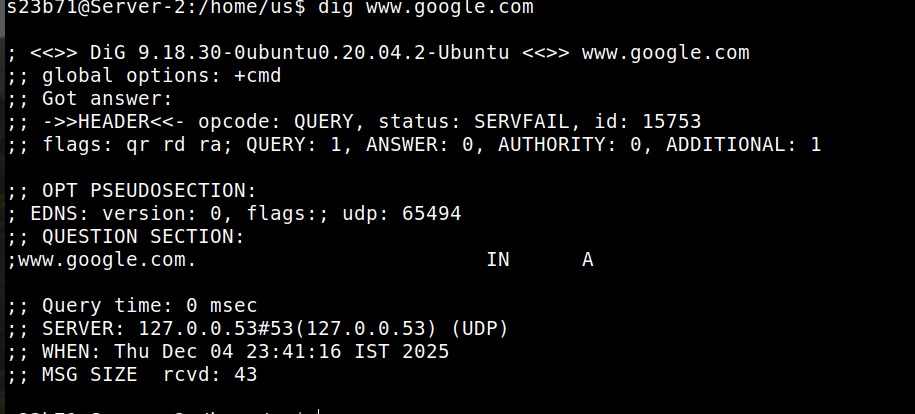
\includegraphics[width=0.90\textwidth]{assets/screenshots/cycle1/dig.png} \\
\textbf{dig} \\[0.35cm]

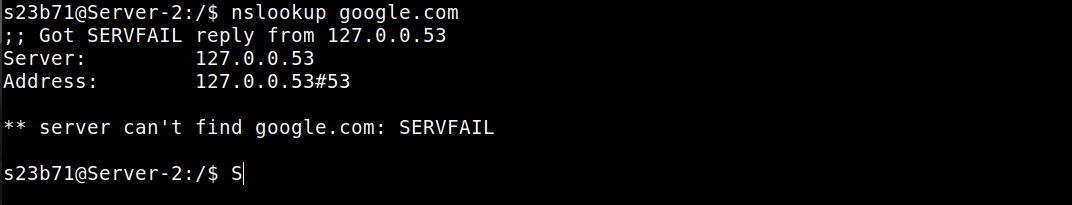
\includegraphics[width=0.90\textwidth]{assets/screenshots/cycle1/nslookup.png} \\
\textbf{nslookup} \\[0.35cm]

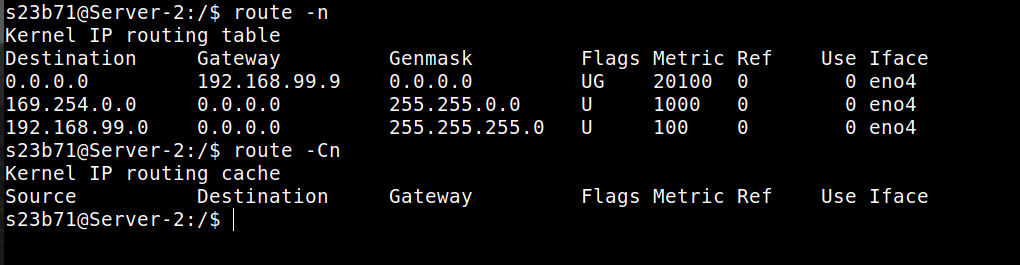
\includegraphics[width=0.90\textwidth]{assets/screenshots/cycle1/route.png} \\
\textbf{route} \\[0.35cm]

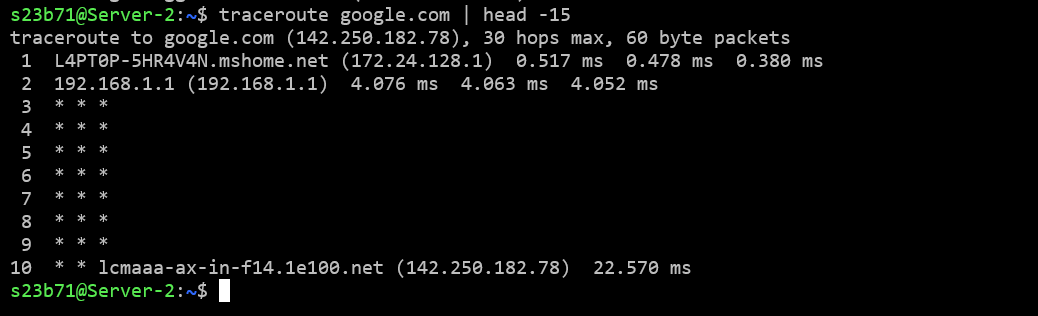
\includegraphics[width=0.90\textwidth]{assets/screenshots/cycle1/traceroute.png} \\
\textbf{traceroute} \\[0.35cm]

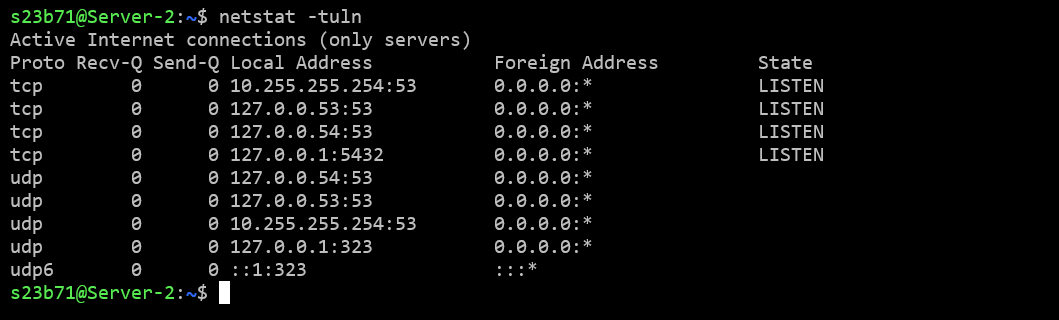
\includegraphics[width=0.90\textwidth]{assets/screenshots/cycle1/netstat.png} \\
\textbf{netstat} \\[0.35cm]

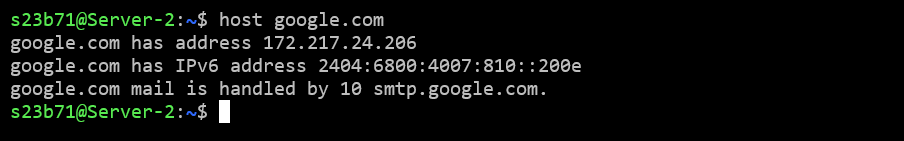
\includegraphics[width=0.90\textwidth]{assets/screenshots/cycle1/host.png} \\
\textbf{host} \\[0.35cm]

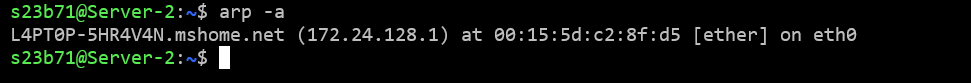
\includegraphics[width=0.90\textwidth]{assets/screenshots/cycle1/arp.png} \\
\textbf{arp} \\[0.35cm]

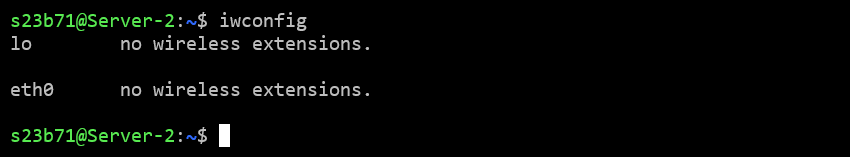
\includegraphics[width=0.90\textwidth]{assets/screenshots/cycle1/iwconfig.png} \\
\textbf{iwconfig} \\[0.35cm]

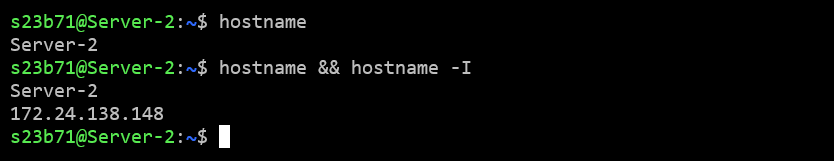
\includegraphics[width=0.90\textwidth]{assets/screenshots/cycle1/hostname.png} \\
\textbf{hostname} \\[0.35cm]

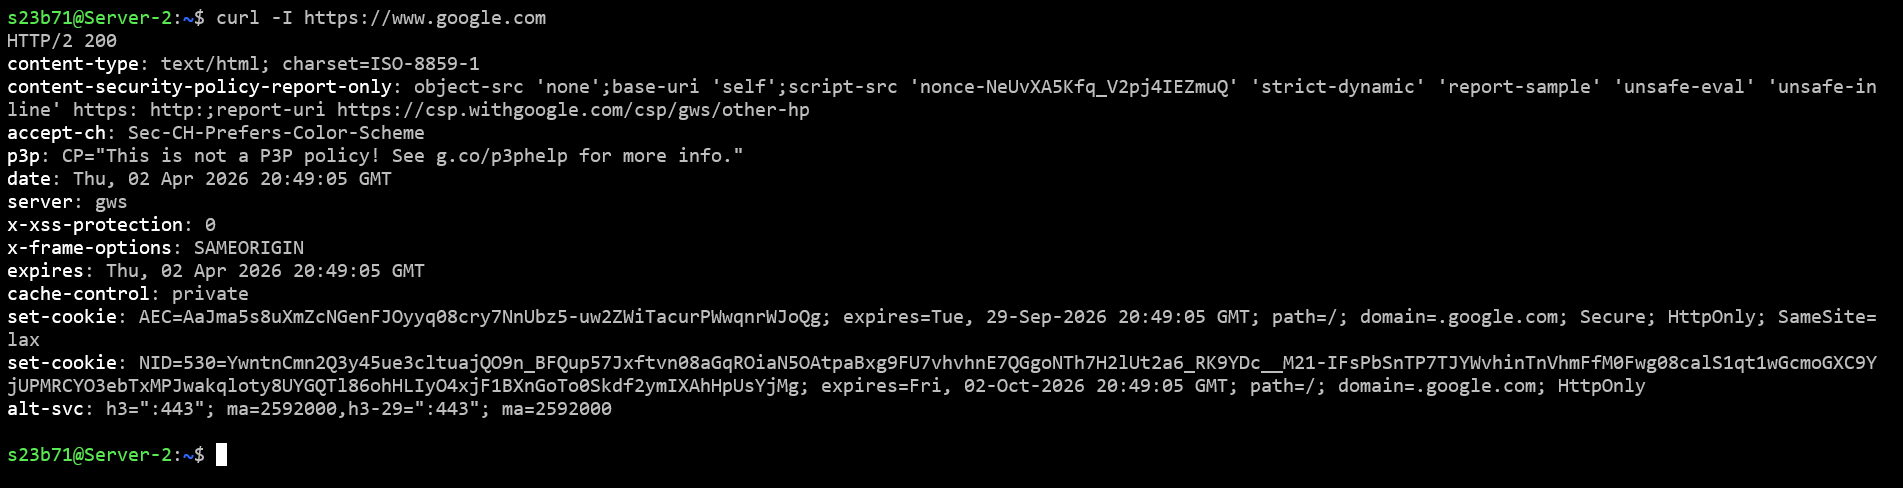
\includegraphics[width=0.90\textwidth]{assets/screenshots/cycle1/curl.png} \\
\textbf{curl} \\[0.35cm]

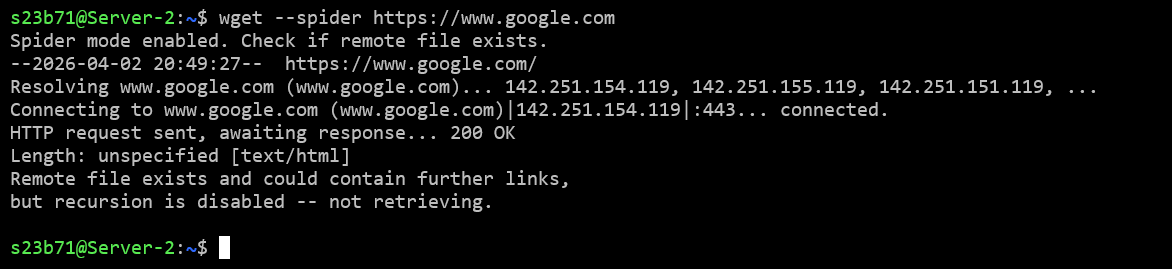
\includegraphics[width=0.90\textwidth]{assets/screenshots/cycle1/wget.png} \\
\textbf{wget} \\[0.35cm]

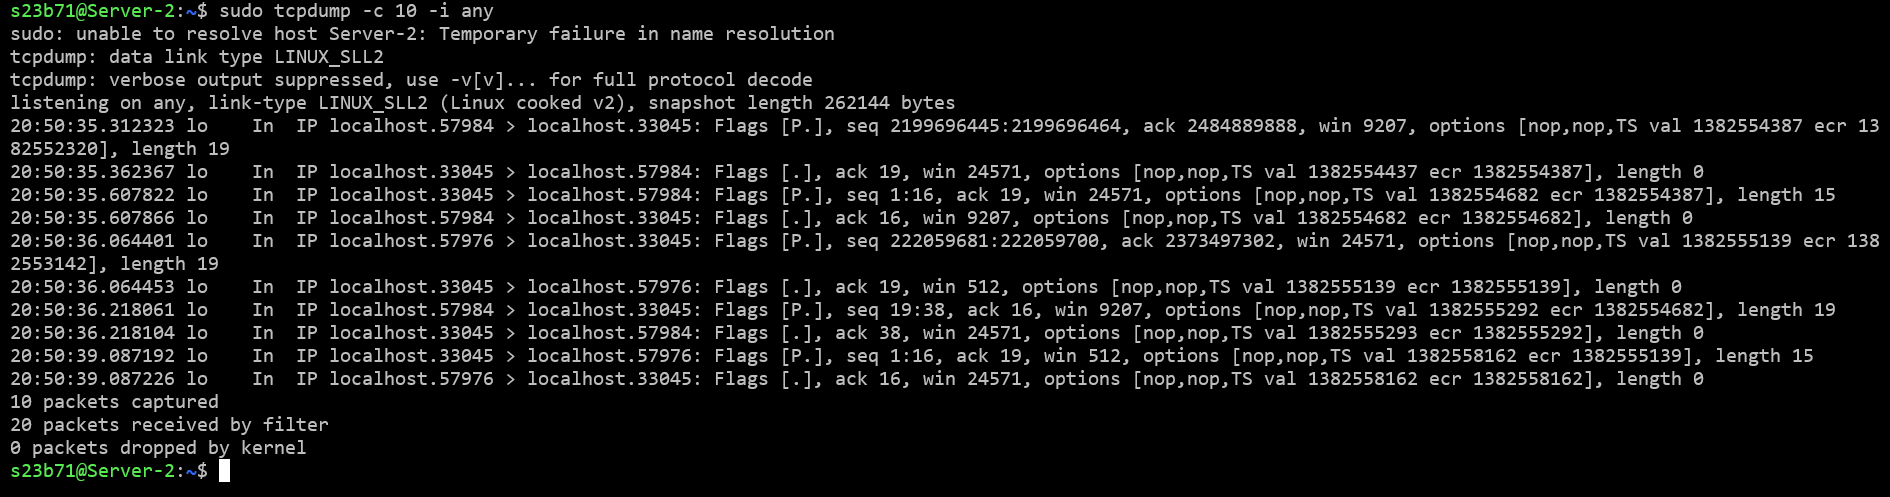
\includegraphics[width=0.90\textwidth]{assets/screenshots/cycle1/tcpdump.png} \\
\textbf{tcpdump} \\[0.35cm]

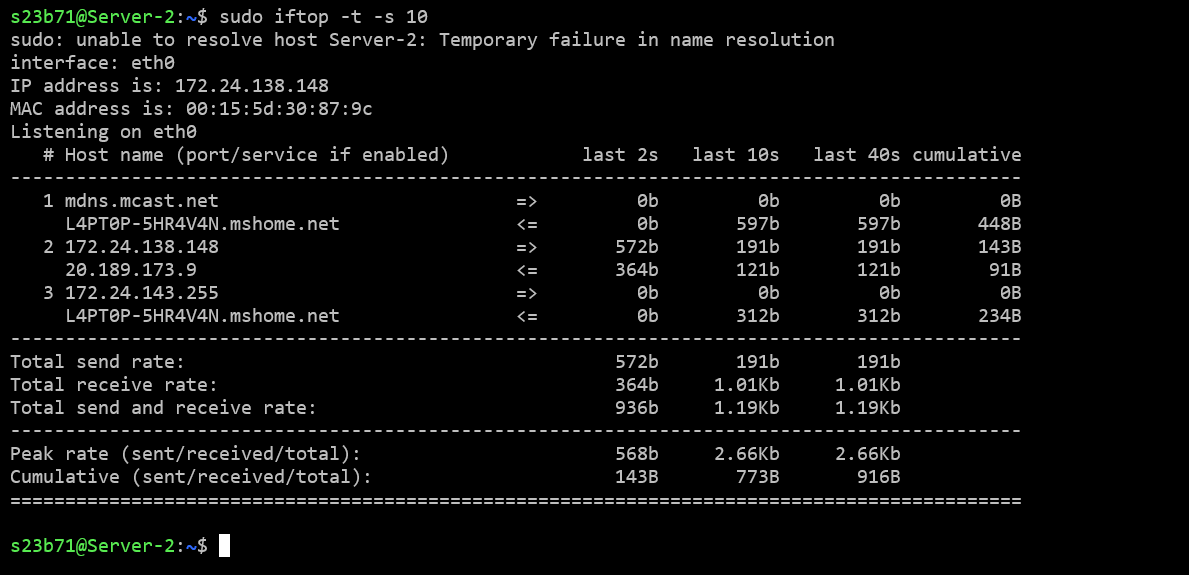
\includegraphics[width=0.90\textwidth]{assets/screenshots/cycle1/iftop.png} \\
\textbf{iftop} \\[0.35cm]

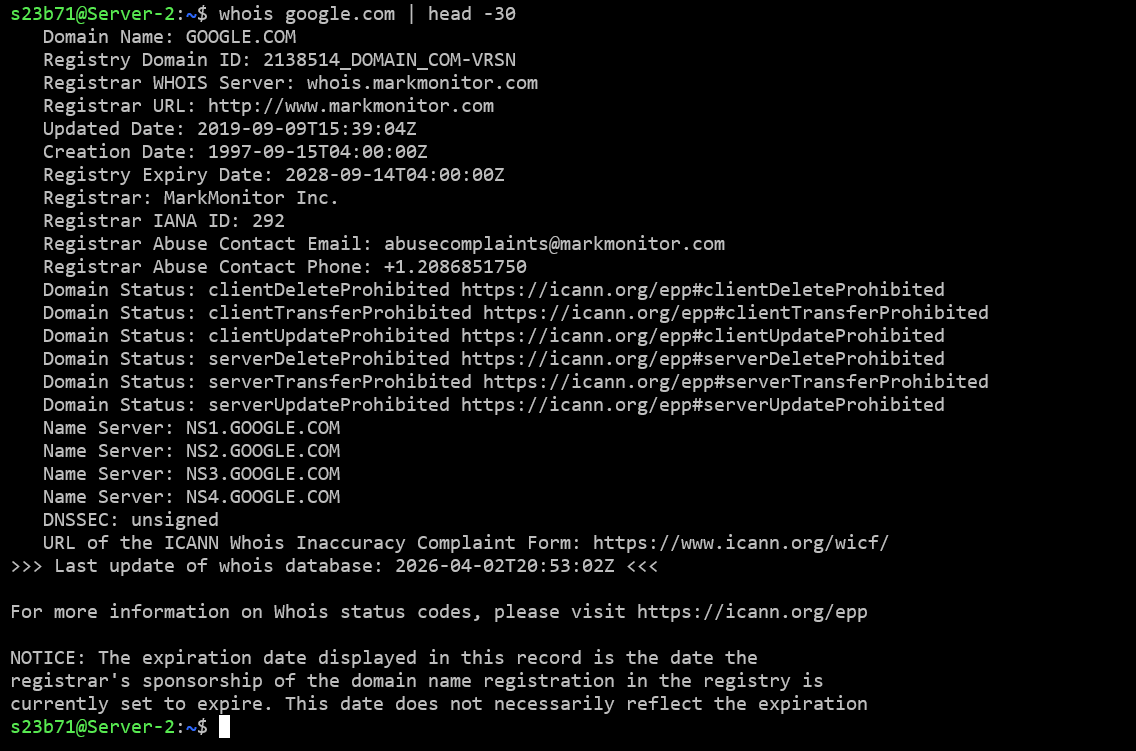
\includegraphics[width=0.90\textwidth]{assets/screenshots/cycle1/whois.png} \\
\textbf{whois} \\[0.35cm]

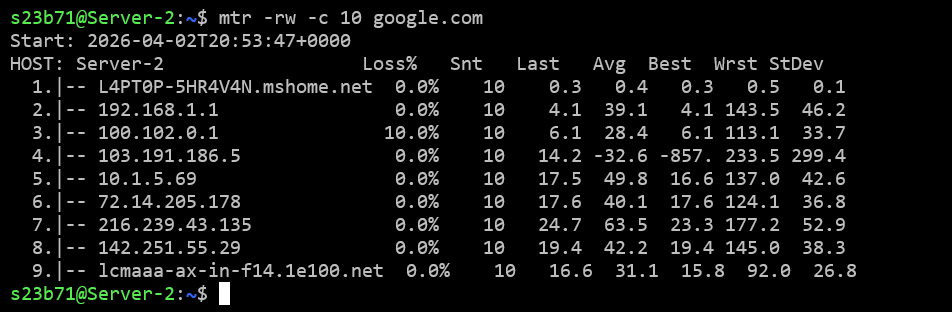
\includegraphics[width=0.90\textwidth]{assets/screenshots/cycle1/mtr.png} \\
\textbf{mtr} \\[0.35cm]

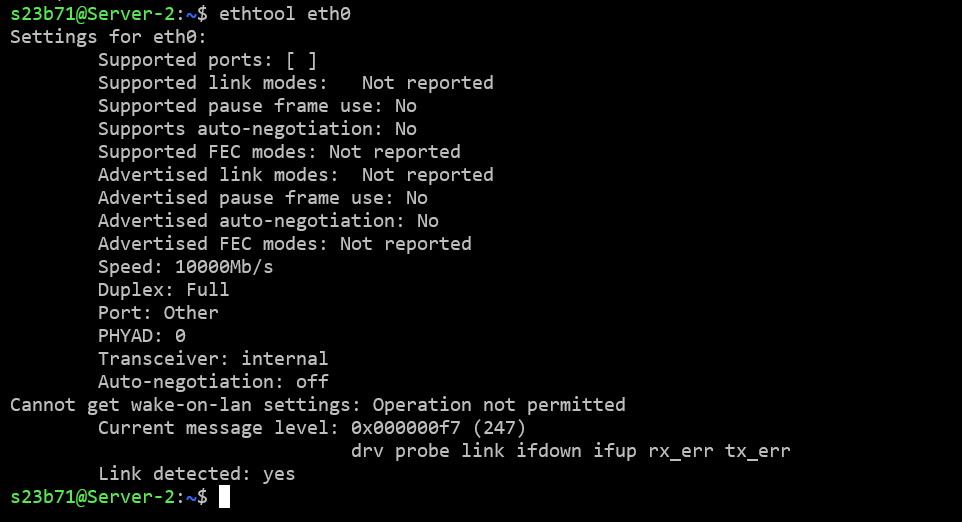
\includegraphics[width=0.90\textwidth]{assets/screenshots/cycle1/ethtool.png} \\
\textbf{ethtool} \\[0.35cm]
\end{center}

\subsection{Result}
The Linux commands related to networking were studied and the outputs for all twenty commands were successfully recorded and analyzed.

%%%%%%%%%% Exp 2 %%%%%%%%%%%%%%%%%%%%%%%%%%%



\experiment{Familiarization of system calls}{19/12/2025}

\subsection{Aim}
To become familiar with Linux system calls.

% ================= A =================
\subsection{A: Array Sum}
\subsubsection{Aim}
Create two processes using \texttt{fork()}. Compute the sum of even numbers in an array in the parent process and the sum of odd numbers in the child process.

\subsubsection{Algorithm}
\begin{enumerate}
    \item Initialize an integer array.
    \item Invoke the \texttt{fork()} system call to spawn a child process.
    \item In the parent process (PID $> 0$), call \texttt{wait(NULL)} to ensure that the child completes first. Then iterate through the array and calculate the sum of even numbers.
    \item In the child process (PID $== 0$), iterate through the array and calculate the sum of odd numbers.
    \item Print the respective sums using \texttt{printf()}.
\end{enumerate}

\subsubsection{Program}
\begin{lstlisting}[language=C]
#include <stdio.h>
#include <sys/types.h>
#include <sys/wait.h>
#include <unistd.h>

int main(void) {
    int arr[] = {1, 2, 3, 4, 5, 6, 7, 8, 9, 10};
    int n = sizeof(arr) / sizeof(arr[0]);
    pid_t pid = fork();

    if (pid < 0) {
        perror("fork");
        return 1;
    }

    if (pid == 0) {
        int odd_sum = 0;
        for (int i = 0; i < n; i++) {
            if (arr[i] % 2 != 0) odd_sum += arr[i];
        }
        printf("Child Process: Odd Sum = %d\n", odd_sum);
    } else {
        int even_sum = 0;
        wait(NULL);
        for (int i = 0; i < n; i++) {
            if (arr[i] % 2 == 0) even_sum += arr[i];
        }
        printf("Parent Process: Even Sum = %d\n", even_sum);
    }
    return 0;
}
\end{lstlisting}
\subsubsection{Output}
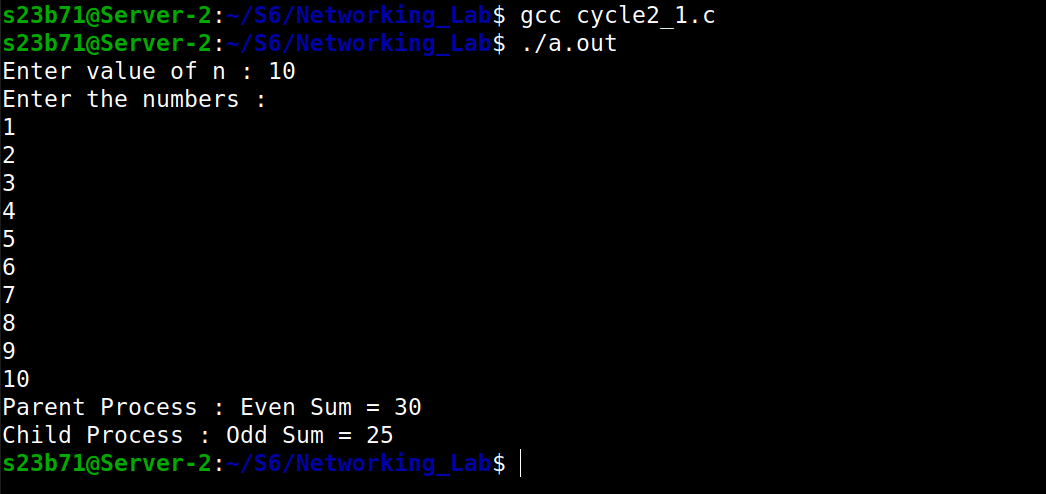
\includegraphics[width=\textwidth]{assets/screenshots/cycle1/system_calls/2_1.png}
% ================= B =================
\subsection{B: Process Identification using Fork}
\subsubsection{Aim}
Write a program to demonstrate process creation and display the process ID (PID) and parent process ID (PPID) for both parent and child processes.

\subsubsection{Algorithm}
\begin{enumerate}
    \item Invoke the \texttt{fork()} system call to spawn a child process.
    \item In the parent block (PID $> 0$), call \texttt{wait(NULL)} to allow the child to execute first. Then use \texttt{getpid()} to print its own ID and \texttt{getppid()} to print the shell's ID.
    \item In the child block (PID $== 0$), use \texttt{getpid()} to print its own unique ID and \texttt{getppid()} to print its parent process ID.
    \item Observe that the child's PPID matches the parent's PID.
\end{enumerate}

\subsubsection{Program}
\begin{lstlisting}[language=C]
#include <stdio.h>
#include <sys/types.h>
#include <sys/wait.h>
#include <unistd.h>

int main(void) {
    pid_t pid = fork();

    if (pid < 0) {
        perror("fork");
        return 1;
    }

    if (pid == 0) {
        printf("Child  -> PID: %d, PPID: %d\n", getpid(), getppid());
    } else {
        wait(NULL);
        printf("Parent -> PID: %d, PPID: %d\n", getpid(), getppid());
    }
    return 0;
}
\end{lstlisting}
\subsubsection{Output}
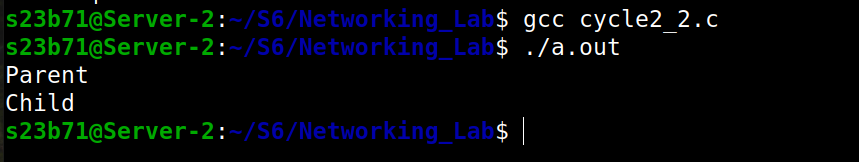
\includegraphics[width=\textwidth]{assets/screenshots/cycle1/system_calls/2_2.png}
% ================= C =================
\subsection{C: File Manipulation System Calls}
\subsubsection{Aim}
Write a C program to implement file manipulation system calls (\texttt{open}, \texttt{write}, \texttt{read}, \texttt{close}).

\subsubsection{Algorithm}
\begin{enumerate}
    \item Invoke \texttt{open()} with flags \texttt{O\_CREAT | O\_RDWR} and permissions \texttt{0777} to create a file.
    \item Use the \texttt{write()} system call to write a string buffer to the file.
    \item Invoke \texttt{close()} to close the file descriptor.
    \item Invoke \texttt{open()} again with the \texttt{O\_RDONLY} flag.
    \item Use the \texttt{read()} system call to fetch bytes from the file descriptor into a local buffer.
    \item Null-terminate the string, print it, and \texttt{close()} the file.
\end{enumerate}

\subsubsection{Program}
\begin{lstlisting}[language=C]
#include <fcntl.h>
#include <stdio.h>
#include <string.h>
#include <sys/stat.h>
#include <sys/types.h>
#include <unistd.h>

int main(void) {
    int fd;
    char write_buf[] = "Linux system calls for file handling";
    char read_buf[100];

    fd = open("exp02_file.txt", O_CREAT | O_RDWR | O_TRUNC, 0777);
    if (fd < 0) {
        perror("open");
        return 1;
    }

    write(fd, write_buf, strlen(write_buf));
    close(fd);

    fd = open("exp02_file.txt", O_RDONLY);
    if (fd < 0) {
        perror("open");
        return 1;
    }

    ssize_t bytes = read(fd, read_buf, sizeof(read_buf) - 1);
    if (bytes < 0) {
        perror("read");
        close(fd);
        return 1;
    }

    read_buf[bytes] = '\0';
    printf("Read from file: %s\n", read_buf);
    close(fd);
    return 0;
}
\end{lstlisting}
\subsubsection{Output}
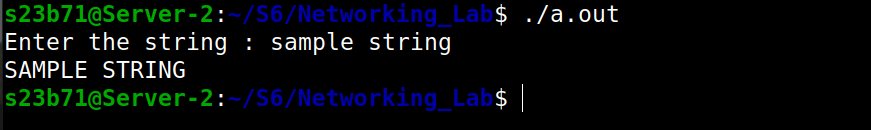
\includegraphics[width=\textwidth]{assets/screenshots/cycle1/system_calls/2_3.png}
\subsection{Result}
The fundamental Linux system calls for process control and file manipulation were successfully studied and implemented.

%%%%%%%%%%%%%%%%%%%%%%%%%%%%%%%%%



\experiment{Socket programming using TCP}{14/01/2026}

\subsection{Aim}
To implement client--server communication using socket programming, with TCP as the transport-layer protocol.

\subsection{Theory}
TCP provides a connection-oriented service because communication occurs through an established connection between a client and a server. TCP is reliable: when a client sends data, acknowledgements are expected from the receiver. If an acknowledgement is not received within a time limit, the data is retransmitted. TCP is a byte-stream protocol and does not preserve message boundaries.

The steps involved in establishing a TCP socket on the server side are as follows:
\begin{itemize}
    \item Create a socket using \texttt{socket()}.
    \item Bind the socket to a local address using \texttt{bind()}.
    \item Listen for incoming connections using \texttt{listen()}.
    \item Accept a client connection using \texttt{accept()}.
    \item Exchange data using \texttt{send()} and \texttt{recv()}.
\end{itemize}

The steps involved in establishing a TCP socket on the client side are as follows:
\begin{itemize}
    \item Create a socket using \texttt{socket()}.
    \item Connect to the server using \texttt{connect()}.
    \item Exchange data using \texttt{send()} and \texttt{recv()}.
\end{itemize}

\subsection{Algorithm}
\noindent\textbf{Server}
\begin{enumerate}
    \item Initialize server IP configuration and port number.
    \item Create a stream socket using \texttt{socket(AF\_INET, SOCK\_STREAM, 0)}.
    \item Bind the socket to the local address with \texttt{bind()}.
    \item Put the socket in passive mode using \texttt{listen()}.
    \item Wait for and accept a client connection using \texttt{accept()}.
    \item Receive client data using \texttt{recv()}.
    \item Process and send response using \texttt{send()}.
    \item Close connected socket and then close the listening socket.
\end{enumerate}

\noindent\textbf{Client}
\begin{enumerate}
    \item Initialize server IP address and port number.
    \item Create a stream socket using \texttt{socket(AF\_INET, SOCK\_STREAM, 0)}.
    \item Establish a connection to the server using \texttt{connect()}.
    \item Transmit a request/message to the server using \texttt{send()}.
    \item Receive server reply using \texttt{recv()}.
    \item Close the socket to terminate communication.
\end{enumerate}

\subsection{Program}
\noindent\textbf{Server Code:}
\lstinputlisting[language=C]{src/cycle2_TCP_server.c}

\noindent\textbf{Client Code:}
\lstinputlisting[language=C]{src/cycle2_TCP_client.c}

\subsection{Output}
\noindent\textbf{\hspace{0.5cm}Server}
\vspace*{0.5cm}

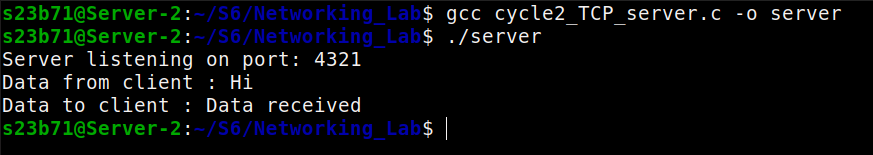
\includegraphics[width=0.95\textwidth]{assets/screenshots/cycle2/1_server.png}

\noindent\textbf{\hspace{0.5cm}Client}
\vspace*{0.5cm}

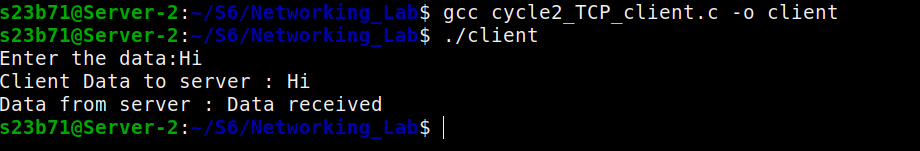
\includegraphics[width=0.95\textwidth]{assets/screenshots/cycle2/1_client.png}

\subsection{Result}
Client--server communication using socket programming and TCP as the transport layer was successfully implemented and verified.

%%%%%%%%%%%%%%%%%%%%%%%%%%%%%%%%%



\experiment{Multi-User Chat Server}{14/01/2026}

\subsection{Aim}
To implement a multi-user chat server using TCP as the transport-layer protocol.

\subsection{Algorithm}
\noindent\textbf{Server}
\begin{enumerate}
    \item Create a TCP socket, bind it to an IP address and port, and listen for incoming connections.
    \item Repeatedly accept new client connections using \texttt{accept()}.
    \item For each connected client, create a separate thread or process for communication.
    \item Receive client messages with \texttt{recv()}.
    \item Broadcast or forward received messages to other clients using \texttt{send()}.
    \item Remove disconnected clients and close their sockets.
\end{enumerate}

\noindent\textbf{Client}
\begin{enumerate}
    \item Create a TCP socket and connect to the server.
    \item Start a background receive loop or thread for incoming chat messages.
    \item Read user input and send messages to the server using \texttt{send()}.
    \item Close the socket on exit.
\end{enumerate}

\subsection{Program}
\noindent\textbf{Server Code:}
\lstinputlisting[language=C]{src/cycle2_TCP_multiserver.c}

\noindent\textbf{Client Code:}
\lstinputlisting[language=C]{src/cycle2_TCP_multiclient.c}

\subsection{Output}
\noindent\textbf{\hspace{0.5cm}Server}
\vspace*{0.5cm}

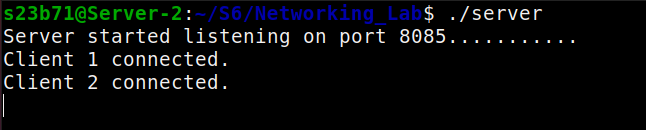
\includegraphics[width=0.95\textwidth]{assets/screenshots/cycle2/2_server.png}

\noindent\textbf{\hspace{0.5cm}Client 1}
\vspace*{0.5cm}

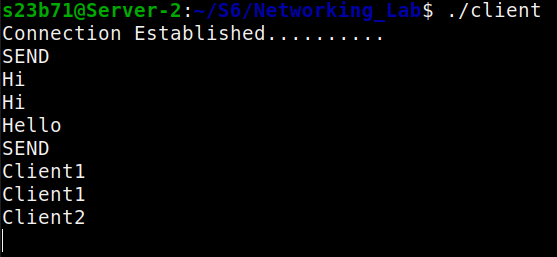
\includegraphics[width=0.95\textwidth]{assets/screenshots/cycle2/2_client1.png}

\noindent\textbf{\hspace{0.5cm}Client 2}
\vspace*{0.5cm}

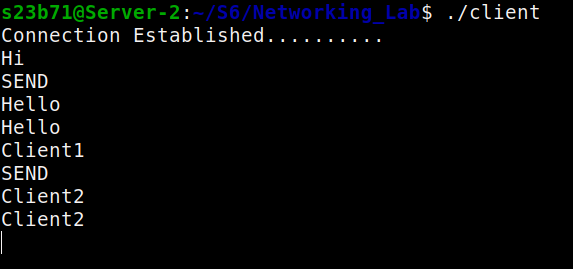
\includegraphics[width=0.95\textwidth]{assets/screenshots/cycle2/2_client2.png}

\subsection{Result}
The multi-user chat server using TCP as the transport layer was implemented and verified successfully using POSIX threads.

%%%%%%%%%%%%%%%%%%%%%%%%%%%%%%%%%



\experiment{Socket Programming Using UDP}{21/01/2026}

\subsection{Aim}
To implement client--server communication using socket programming, with UDP as the transport-layer protocol.

\subsection{Algorithm}
\noindent\textbf{Server}
\begin{enumerate}
    \item Initialize the server IP address and port number.
    \item Create a UDP socket using \texttt{socket(AF\_INET, SOCK\_DGRAM, 0)}.
    \item Bind the socket to the local address using \texttt{bind()}.
    \item Receive a datagram from a client using \texttt{recvfrom()}.
    \item Process the request and send a reply using \texttt{sendto()}.
    \item Close the socket.
\end{enumerate}

\noindent\textbf{Client}
\begin{enumerate}
    \item Initialize the server IP address and port number.
    \item Create a UDP socket.
    \item Send a message to the server using \texttt{sendto()}.
    \item Receive the server response using \texttt{recvfrom()}.
    \item Close the socket.
\end{enumerate}

\subsection{Program}
\noindent\textbf{Server Code:}
\lstinputlisting[language=C]{src/cycle2_UDP_server.c}

\noindent\textbf{Client Code:}
\lstinputlisting[language=C]{src/cycle2_UDP_client.c}

\subsection{Output}
\noindent\textbf{\hspace{0.5cm}Server}
\vspace*{0.5cm}

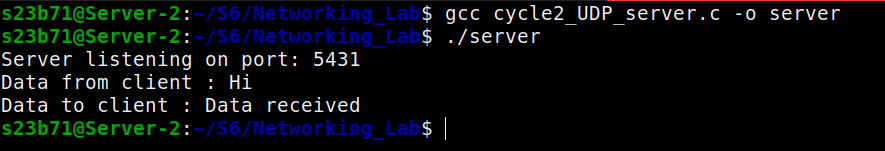
\includegraphics[width=0.95\textwidth]{assets/screenshots/cycle2/3_server.png}

\noindent\textbf{\hspace{0.5cm}Client}
\vspace*{0.5cm}

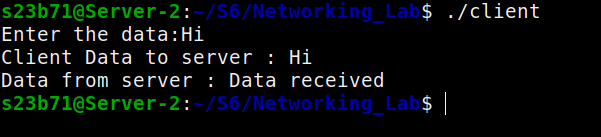
\includegraphics[width=0.95\textwidth]{assets/screenshots/cycle2/3_client.png}

\subsection{Result}
Client--server communication using the UDP protocol was successfully implemented and verified.

%%%%%%%%%%%%%%%%%%%%%%%%%%%%%%%%%



\experiment{Concurrent Time Server}{21/01/2026}

\subsection{Aim}
To implement a concurrent time-server application using UDP on a remote server. The client sends a time request to the server, the server sends its system time back to the client, and the client displays the result.

\subsection{Algorithm}
\noindent\textbf{Server}
\begin{enumerate}
    \item Create a UDP socket and bind it to the server address and port.
    \item Wait for a client request using \texttt{recvfrom()}.
    \item Handle each request concurrently (for example, using a child process or thread).
    \item Fetch the current system time using \texttt{time()} and \texttt{ctime()}.
    \item Send the time string back to the requesting client using \texttt{sendto()}.
\end{enumerate}

\noindent\textbf{Client}
\begin{enumerate}
    \item Create a UDP socket.
    \item Send a \texttt{"time"} request to the server.
    \item Receive the returned time string using \texttt{recvfrom()}.
    \item Display the received time and close the socket.
\end{enumerate}

\subsection{Program}
\noindent\textbf{Server Code:}
\lstinputlisting[language=C]{src/cycle2_UDP_timeserver.c}

\noindent\textbf{Client Code:}
\lstinputlisting[language=C]{src/cycle2_UDP_timeclient.c}

\subsection{Output}
\noindent\textbf{\hspace{0.5cm}Server}
\vspace*{0.5cm}

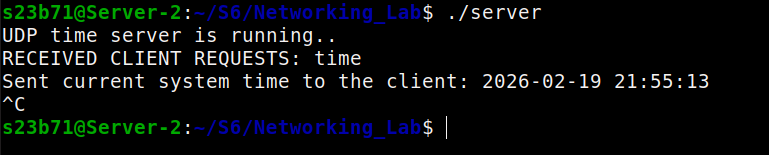
\includegraphics[width=0.95\textwidth]{assets/screenshots/cycle2/4_server.png}

\noindent\textbf{\hspace{0.5cm}Client}
\vspace*{0.5cm}

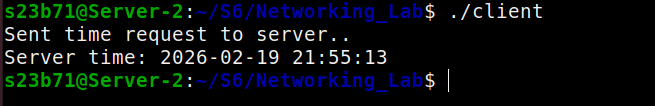
\includegraphics[width=0.95\textwidth]{assets/screenshots/cycle2/4_client.png}

\subsection{Result}
The concurrent time server was implemented using the UDP protocol and verified successfully.

%%%%%%%%%%%%%%%%%%%%%%%%%%%%%%%%%



\experiment{File Transfer Protocol}{06/02/2026}

\subsection{Aim}
To develop a concurrent file server that provides a file requested by a client if it exists. If not, the server sends an appropriate message to the client. The server should also send its process ID (PID) to clients for display along with file content or status messages.

\subsection{Theory}
FTP stands for File Transfer Protocol. It is a standard Internet protocol provided by TCP/IP and used to transfer files from one host to another. It is commonly used for transferring web page files from their creator to the computer that acts as a server for other computers on the Internet. It is also used to download files from remote servers.

\subsection{Algorithm}
\noindent\textbf{Server}
\begin{enumerate}
    \item Create a TCP socket, bind it to an address, and listen.
    \item Accept a client connection.
    \item Receive commands using \texttt{recv()}.
    \item For \texttt{GET}, open the requested file and send its contents; send an error if the file is absent.
    \item For \texttt{PUT}, receive data and write it to the destination file.
    \item For \texttt{BYE}, close the client and server sockets, then terminate.
\end{enumerate}

\noindent\textbf{Client}
\begin{enumerate}
    \item Create a TCP socket and connect to the server.
    \item Send commands (GET/PUT/BYE) with required parameters.
    \item For \texttt{GET}, receive file/status data and store or display the result.
    \item For \texttt{PUT}, read a local file and send data to the server.
    \item For \texttt{BYE}, close the socket and exit.
\end{enumerate}

\subsection{Program}
\noindent\textbf{Server Code:}
\lstinputlisting[language=C]{src/cycle2_ftp_server.c}

\noindent\textbf{Client Code:}
\lstinputlisting[language=C]{src/cycle2_ftp_client.c}

\subsection{Output}
\noindent\textbf{\hspace{0.5cm}Server}
\vspace*{0.5cm}

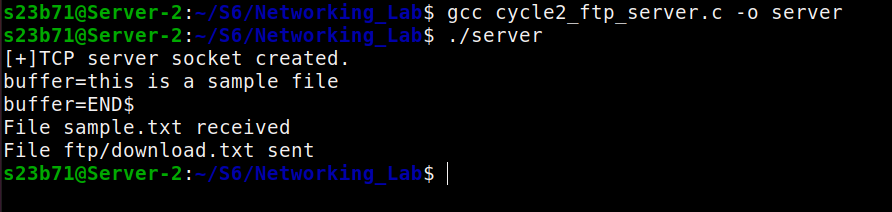
\includegraphics[width=0.95\textwidth]{assets/screenshots/cycle2/5_server.png}

\noindent\textbf{\hspace{0.5cm}Client}
\vspace*{0.5cm}

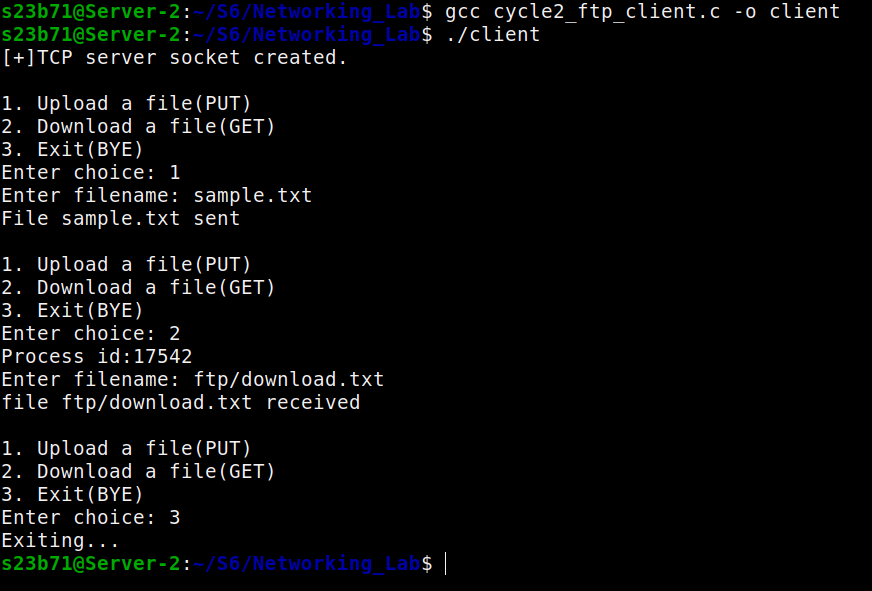
\includegraphics[width=0.95\textwidth]{assets/screenshots/cycle2/5_client.png}

\subsection{Result}
The FTP server was successfully implemented with \texttt{GET}, \texttt{PUT}, and \texttt{BYE} handling, along with PID reporting in server responses.

%%%%%%%%%%%%%%%%%%%%%%%%%%%%%%%%%



\experiment{Stop-and-Wait flow control protocol}{06/02/2026}

\subsection{Aim}
To implement a simple Stop-and-Wait flow-control protocol using client--server datagram sockets.

\subsection{Theory}
Stop-and-Wait is a data-link-layer protocol used for transmission over noiseless channels. It provides unidirectional data transmission, meaning that either sending or receiving takes place at a given time. It provides flow control but does not provide error control.
The sender transmits one packet at a time and waits for an acknowledgment before sending the next packet. On the receiver side, each received packet is processed and acknowledged.

\subsection{Algorithm}
\noindent\textbf{Server (Receiver)}
\begin{enumerate}
    \item Receive one data frame.
    \item Send acknowledgment for the received frame.
    \item Repeat for all frames.
\end{enumerate}

\noindent\textbf{Client (Sender)}
\begin{enumerate}
    \item Initialize frame sequence.
    \item Send one frame.
    \item Wait for corresponding ACK.
    \item On ACK reception, send next frame.
    \item Continue until all frames are sent.
\end{enumerate}

\subsection{Program}
\noindent\textbf{Server Code:}
\lstinputlisting[language=C]{src/cycle3_stop_and_wait_server.c}

\noindent\textbf{Client Code:}
\lstinputlisting[language=C]{src/cycle3_stop_and_wait_client.c}

\subsection{Output}
\noindent\textbf{\hspace{0.5cm}Server}
\vspace*{0.5cm}


\includegraphics[width=0.95\textwidth]{assets/screenshots/cycle3/1_server.png}

\noindent\textbf{\hspace{0.5cm}Client}
\vspace*{0.5cm}


\includegraphics[width=0.95\textwidth]{assets/screenshots/cycle3/1_client.png}

\subsection{Result}
The Simple Stop-and-Wait flow control protocol was successfully implemented and verified over UDP.

%%%%%%%%%%%%%%%%%%%%%%%%%%%%%%%%%



\experiment{Stop-and-Wait ARQ flow control protocol}{06/02/2026}

\subsection{Aim}
To implement the Stop-and-Wait Automatic Repeat reQuest (ARQ) protocol with a timeout mechanism.

\subsection{Theory}
Stop-and-Wait ARQ extends Stop-and-Wait by adding error control. The sender maintains a timeout value. If an acknowledgment is not received within the specified time after a packet is sent, the same packet is retransmitted. On the receiver side, the packet is processed and an acknowledgment is sent.

\subsection{Algorithm}
\noindent\textbf{Server (Receiver)}
\begin{enumerate}
    \item Receive frames from the sender.
    \item If frame is valid, send ACK (optionally simulate ACK loss for testing).
    \item Ignore duplicates appropriately.
\end{enumerate}

\noindent\textbf{Client (Sender)}
\begin{enumerate}
    \item Send frame and start timeout timer.
    \item Wait for ACK.
    \item If an ACK arrives before timeout, send the next frame.
    \item If timeout occurs, retransmit the same frame.
    \item Repeat until all frames are acknowledged.
\end{enumerate}

\subsection{Program}
\noindent\textbf{Server Code:}
\lstinputlisting[language=C]{src/cycle3_stop_and_wait_ARQ_server.c}

\noindent\textbf{Client Code:}
\lstinputlisting[language=C]{src/cycle3_stop_and_wait_ARQ_client.c}

\subsection{Output}
\noindent\textbf{\hspace{0.5cm}Server}
\vspace*{0.5cm}


\includegraphics[width=0.95\textwidth]{assets/screenshots/cycle3/2_server.png}

\noindent\textbf{\hspace{0.5cm}Client}
\vspace*{0.5cm}

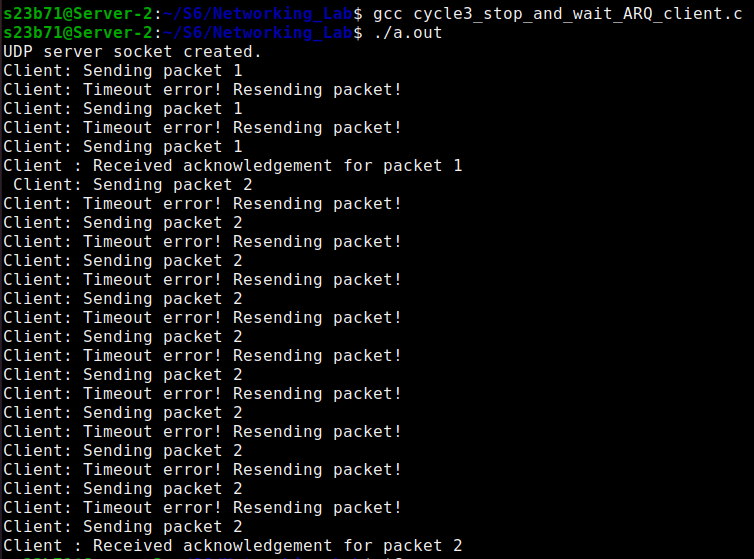
\includegraphics[width=0.95\textwidth]{assets/screenshots/cycle3/2_client.png}

\subsection{Result}
The Stop-and-Wait ARQ protocol was successfully implemented with timeout-based retransmission logic.

%%%%%%%%%%%%%%%%%%%%%%%%%%%%%%%%%



\experiment{Go-Back-N ARQ flow control protocol}{06/02/2026}

\subsection{Aim}
To implement the Go-back-N ARQ protocol using a sliding window strategy over UDP.

\subsection{Theory}
Go-Back-N ARQ is a sliding-window protocol. Up to \(N\) packets can be sent before receiving acknowledgments, where \(N\) is the window size. In Go-Back-N ARQ, the sender window size is \(N\) and the receiver window size is 1. If an acknowledgment is not received within the agreed timeout period, all frames in the current window are retransmitted. After acknowledgment of a packet, the window slides forward by one position. This process continues until all packets are transmitted. Corrupted or out-of-order frames are discarded.

\subsection{Algorithm}
\noindent\textbf{Server (Receiver)}
\begin{enumerate}
    \item Receive incoming frames and verify expected sequence.
    \item Accept in-order frame and send cumulative ACK.
    \item Discard out-of-order frames and repeat ACK of last in-order frame.
\end{enumerate}

\noindent\textbf{Client (Sender)}
\begin{enumerate}
    \item Initialize frame list, base, and window size.
    \item Send all frames in current window.
    \item Wait for ACKs.
    \item On valid ACK, slide window forward.
    \item On timeout, retransmit frames from base onward.
    \item Continue until all frames are acknowledged.
\end{enumerate}

\subsection{Program}
\noindent\textbf{Server Code:}
\lstinputlisting[language=C]{src/cycle3_gobackn_server.c}

\noindent\textbf{Client Code:}
\lstinputlisting[language=C]{src/cycle3_gobackn_client.c}

\subsection{Output}
\noindent\textbf{\hspace{0.5cm}Server}
\vspace*{0.5cm}


\includegraphics[width=0.95\textwidth]{assets/screenshots/cycle3/3_server.png}

\noindent\textbf{\hspace{0.5cm}Client}
\vspace*{0.5cm}


\includegraphics[width=0.95\textwidth]{assets/screenshots/cycle3/3_client.png}

\subsection{Result}
The Go-back-N ARQ protocol was successfully implemented for sliding window transmission.

%%%%%%%%%%%%%%%%%%%%%%%%%%%%%%%%%



\experiment{Selective Repeat ARQ Flow Control Protocol}{20/02/2026}

\subsection{Aim}
To implement Selective Repeat ARQ, where only lost or damaged frames are retransmitted.

\subsection{Theory}
In Selective Repeat ARQ, the sender transmits multiple frames within a window without waiting for individual acknowledgment after every frame, unlike Stop-and-Wait. Only lost or damaged frames are retransmitted, while correctly received frames are buffered even if they arrive out of order. The receiver tracks sequence numbers and can send negative acknowledgment (NACK) for missing or damaged frames. The sender retransmits only the required frames.

\subsection{Algorithm}
\noindent\textbf{Server (Receiver)}
\begin{enumerate}
    \item Receive frames and buffer valid ones.
    \item Send individual ACK for correctly received frames.
    \item Send NACK (or withhold ACK) for missing/corrupted frames.
\end{enumerate}

\noindent\textbf{Client (Sender)}
\begin{enumerate}
    \item Send frames within current window.
    \item Maintain ACK status for each frame.
    \item Retransmit only frames that are unacknowledged/NACKed after timeout.
    \item Slide window when lower sequence frames are acknowledged.
    \item Continue until all frames are delivered.
\end{enumerate}

\subsection{Program}
\noindent\textbf{Client Code:}
\lstinputlisting[language=C]{src/cycle3_selective_ARQ_client.c}

\noindent\textbf{Server Code:}
\lstinputlisting[language=C]{src/cycle3_selective_ARQ_server.c}

\subsection{Output}
\begin{center}

\includegraphics[width=0.95\textwidth]{assets/screenshots/cycle3/3_server.png}\\[0.2cm]

\includegraphics[width=0.95\textwidth]{assets/screenshots/cycle3/3_client.png}
\end{center}

\subsection{Result}
The Selective Repeat ARQ protocol was successfully implemented using retransmission of only unacknowledged packets.

%%%%%%%%%%%%%%%%%%%%%%%%%%%%%%%%%



\experiment{Distance Vector Routing Protocol}{20/02/2026}

\subsection{Aim}
To implement and simulate the Distance Vector Routing protocol.

\subsection{Theory}
Distance Vector Routing is a dynamic routing approach used to identify the shortest path between nodes in a network. Each router shares its routing information with neighboring routers. Neighboring routers use this information to update their own routing tables. The Bellman--Ford algorithm is used to compute shortest paths.

\subsection{Algorithm}
\begin{enumerate}
    \item Initialize each router's distance vector from local link costs.
    \item Exchange distance vectors with neighboring routers.
    \item Update route to destination \(C\) via neighbor \(B\) using:
    \(D(A,C)=\min(D(A,C), D(A,B)+D(B,C))\).
    \item If any entry changes, propagate updated vector.
    \item Repeat until no table updates occur (network converges).
\end{enumerate}

\subsection{Program}
\lstinputlisting[language=C]{src/cycle4_DVR.c}

\subsection{Output}
\begin{center}

\includegraphics[width=0.75\textwidth]{assets/screenshots/cycle4/1.png}\\[0.2cm]
\textbf{Distance Vector Routing Program Output}
\end{center}

\subsection{Result}
The Distance Vector Routing algorithm was successfully simulated using the Bellman-Ford approach.

%%%%%%%%%%%%%%%%%%%%%%%%%%%%%%%%%



\experiment{Link State Routing protocol}{20/02/2026}

\subsection{Aim}
To implement and simulate the Link State Routing protocol utilizing Dijkstra's shortest path algorithm.

\subsection{Theory}
Link State Routing is a method in which each router shares knowledge of its neighboring links with other routers in the network. In this algorithm, each router builds an understanding of the full network topology and then constructs its routing table based on that topology. Each router shares connection-state data with its neighbors, which in turn propagate the data further, until all routers have a complete topology view. Dijkstra's algorithm is then used to compute shortest paths.

\subsection{Algorithm}
\begin{enumerate}
    \item Choose source router and initialize visited set.
    \item Assign tentative distances: 0 to source, direct-link costs to neighbors, infinity to others.
    \item Select unvisited node with smallest tentative distance.
    \item Mark it visited and relax distances of adjacent unvisited nodes.
    \item Repeat until all nodes are visited.
    \item Construct routing entries from computed shortest paths.
\end{enumerate}

\subsection{Program}
\lstinputlisting[language=C]{src/cycle4_LSR.c}

\subsection{Output}
\begin{center}

\includegraphics[width=0.75\textwidth]{assets/screenshots/cycle4/2.png}\\[0.2cm]
\textbf{Link State Routing Program Output}
\end{center}

\subsection{Result}
Link State Routing using Dijkstra's algorithm was successfully simulated.

%%%%%%%%%%%%%%%%%%%%%%%%%%%%%%%%%



\experiment{Leaky Bucket}{20/02/2026}

\subsection{Aim}
To implement the Leaky Bucket algorithm for congestion control.

\subsection{Theory}
The Leaky Bucket is a congestion-control algorithm used to maintain a constant rate of data flow in a network. Consider a bucket with a hole at the bottom: regardless of the rate at which water is poured in, water exits at a nearly constant rate. If the bucket becomes full, excess water overflows. This is the principle behind the Leaky Bucket method. In networking, outgoing packets are placed into a logical bucket and transmitted at a fixed rate. If the bucket is full, newly arriving packets are dropped.

\subsection{Algorithm}
\begin{enumerate}
    \item Initialize bucket capacity and constant leak rate.
    \item On packet arrival, add it if free capacity exists.
    \item If bucket is full, drop/overflow that packet.
    \item Periodically transmit data at fixed leak rate.
    \item Update remaining bucket content and repeat.
\end{enumerate}

\subsection{Program}
\lstinputlisting[language=C]{src/cycle5_leaky_bucket.c}

\subsection{Output}
\begin{center}

\includegraphics[width=0.75\textwidth]{assets/screenshots/cycle5/1.png}\\[0.2cm]
\textbf{Leaky Bucket Program Output}
\end{center}

\subsection{Result}
Congestion control via the leaky bucket algorithm was successfully implemented.

%%%%%%%%%%%%%%%%%%%%%%%%%%%%%%%%%



\experiment{Understanding the Wireshark Tool}{27/02/2026}

\subsection{Aim}
To understand the usage of the Wireshark packet analyzer tool.

\subsection{Theory}
Wireshark is an open-source network analyzer that captures packets from a network connection, such as the connection between your computer and the internet. A packet is a discrete unit of data in a typical Ethernet network. Wireshark is used for network troubleshooting and communication-protocol analysis. It captures network packets in real time and displays them in a human-readable format. It provides advanced features including live capture, offline analysis, a three-pane packet browser, and coloring rules for analysis. Wireshark captures network traffic from Ethernet, Bluetooth, Wireless (IEEE 802.11), Token Ring, Frame Relay, and other connection types.

Wireshark provides three major capabilities:
\begin{itemize}
    \item \textbf{Packet Capture:} Wireshark listens to a network connection in real time and captures streams of traffic.
    \item \textbf{Filtering:} Wireshark can filter captured data so that only relevant packets are displayed.
    \item \textbf{Visualization:} Wireshark allows detailed packet inspection and visualization of complete conversations and network streams.
\end{itemize}

\subsection{Execution Steps}
\begin{itemize}
    \item Install Wireshark using \texttt{sudo apt install wireshark}.
    \item Select the active network interface and start packet capture.
    \item Open a web browser to generate HTTP and DNS traffic.
    \item Apply the following display filters in the Wireshark filter bar:
    \begin{itemize}
        \item \textbf{TCP SYN:} \texttt{tcp.flags.syn == 1 \&\& tcp.flags.ack == 0}
        \item \textbf{TCP SYN-ACK:} \texttt{tcp.flags.syn == 1 \&\& tcp.flags.ack == 1}
        \item \textbf{HTTP:} \texttt{http}
        \item \textbf{DNS:} \texttt{dns}
    \end{itemize}
    \item Observe the Statistics $\rightarrow$ Flow Graph to visualize the TCP connection lifecycle.
\end{itemize}

\subsection{Output}
\begin{center}
\textbf{A. Three-Way Handshaking and Connection Termination}\\[0.3cm]
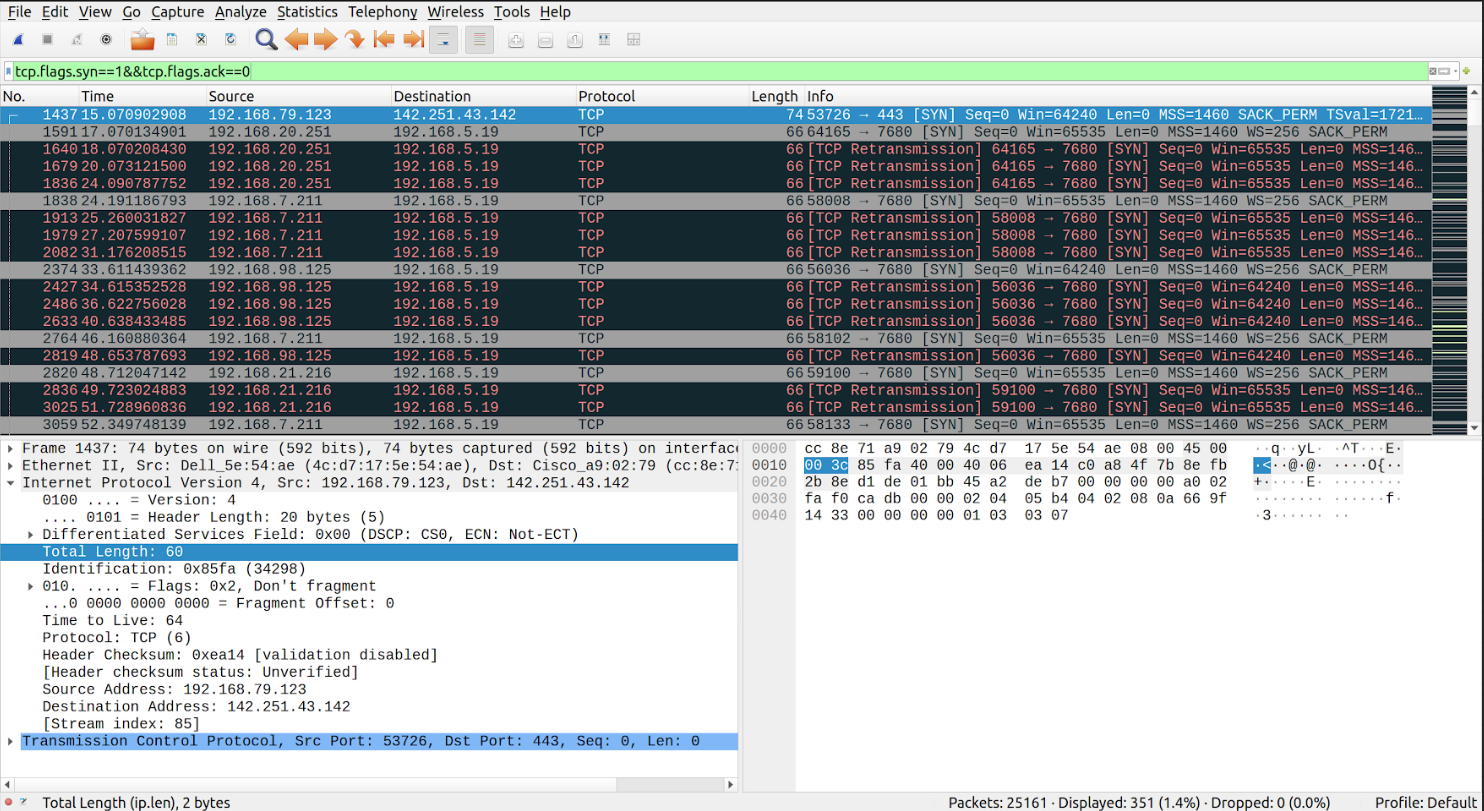
\includegraphics[width=0.8\textwidth]{assets/images/exp15/1.png}\\
\textbf{TCP SYN packet} (\texttt{tcp.flags.syn == 1 \&\& tcp.flags.ack == 0})\\[0.4cm]
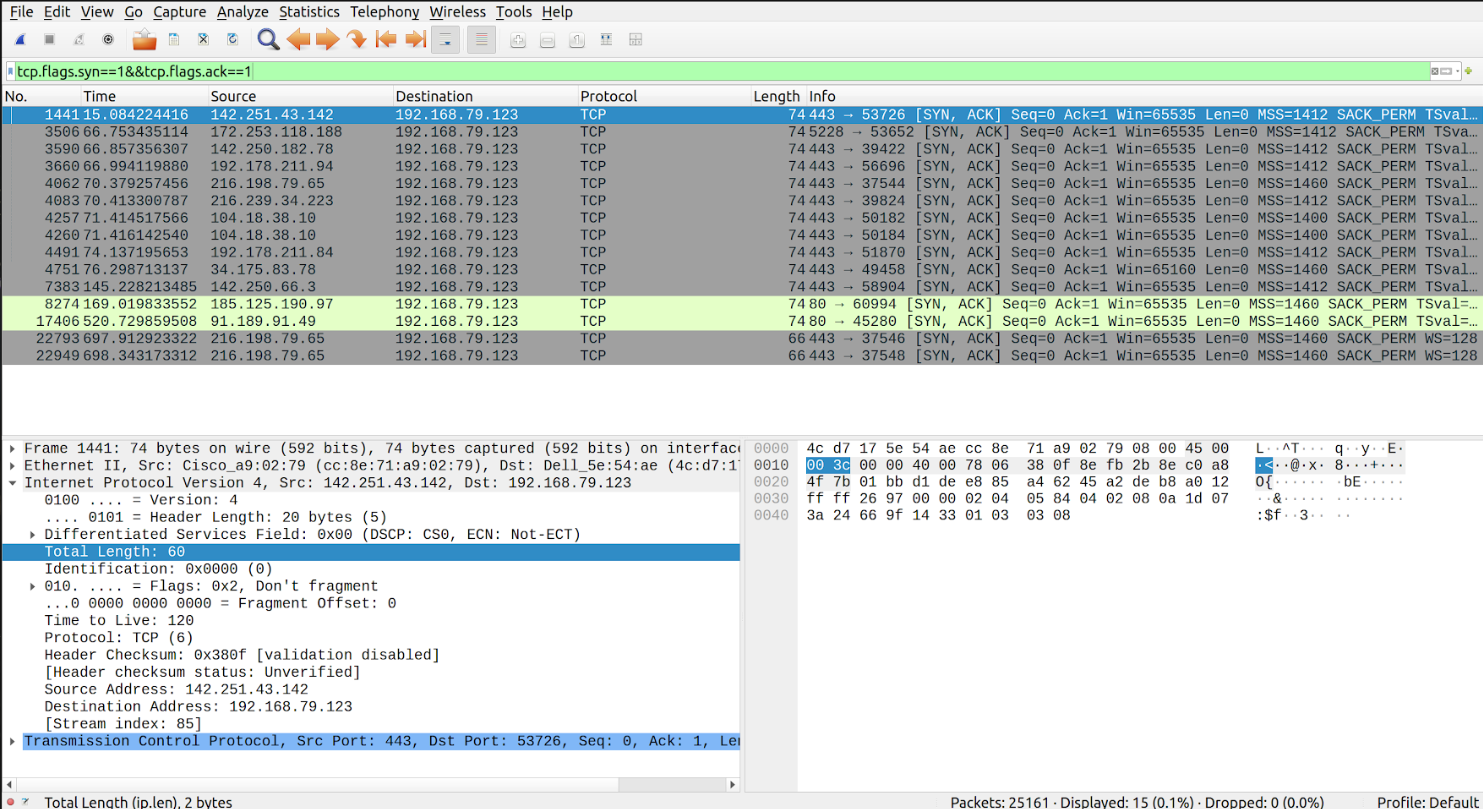
\includegraphics[width=0.8\textwidth]{assets/images/exp15/4.png}\\
\textbf{TCP SYN-ACK packet} (\texttt{tcp.flags.syn == 1 \&\& tcp.flags.ack == 1})\\[0.4cm]
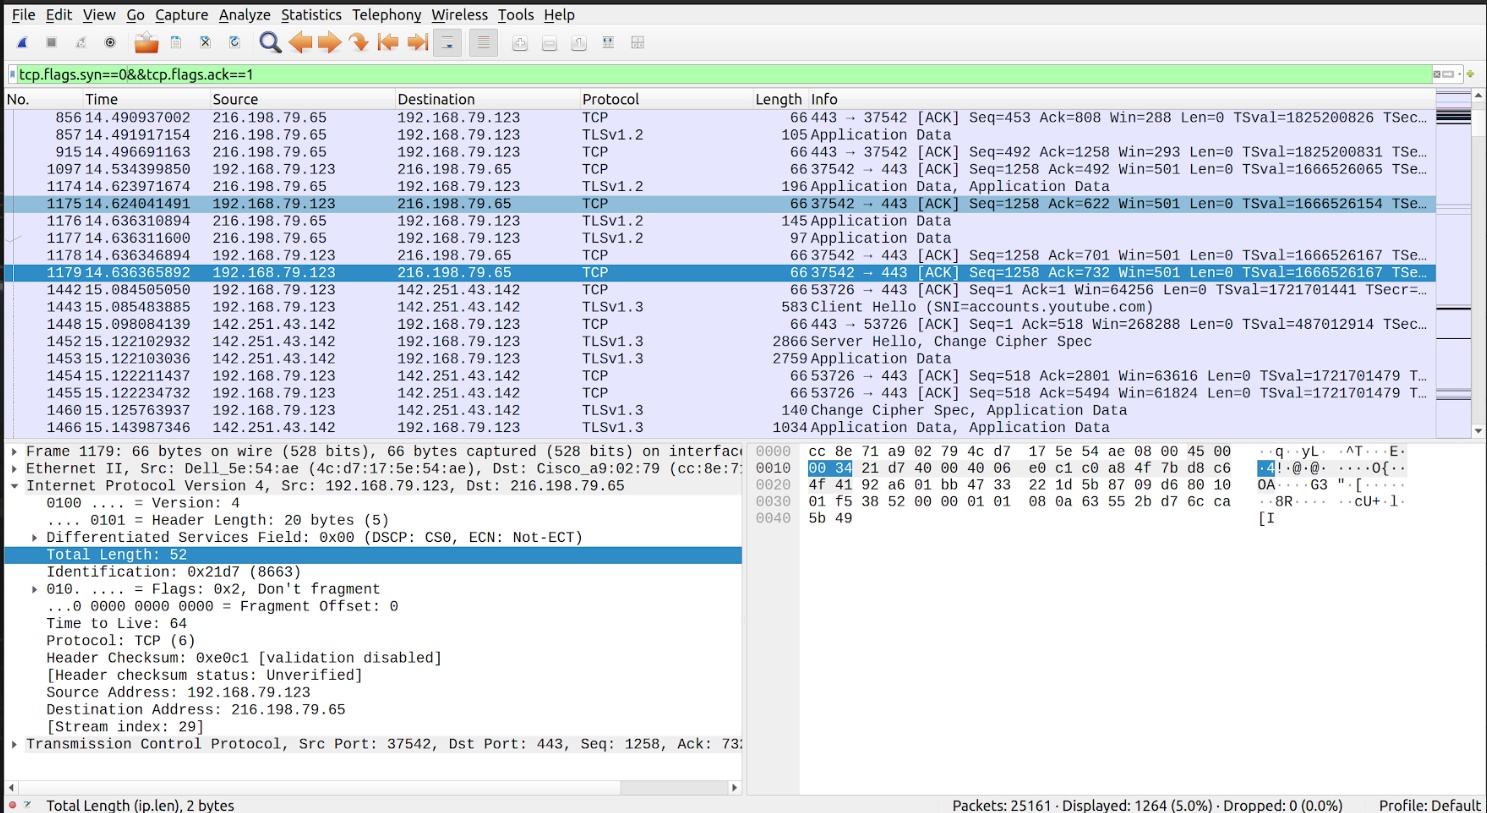
\includegraphics[width=0.8\textwidth]{assets/images/exp15/5.png}\\
\textbf{TCP ACK packet} (\texttt{tcp.flags.syn == 0 \&\& tcp.flags.ack == 1})\\[0.4cm]
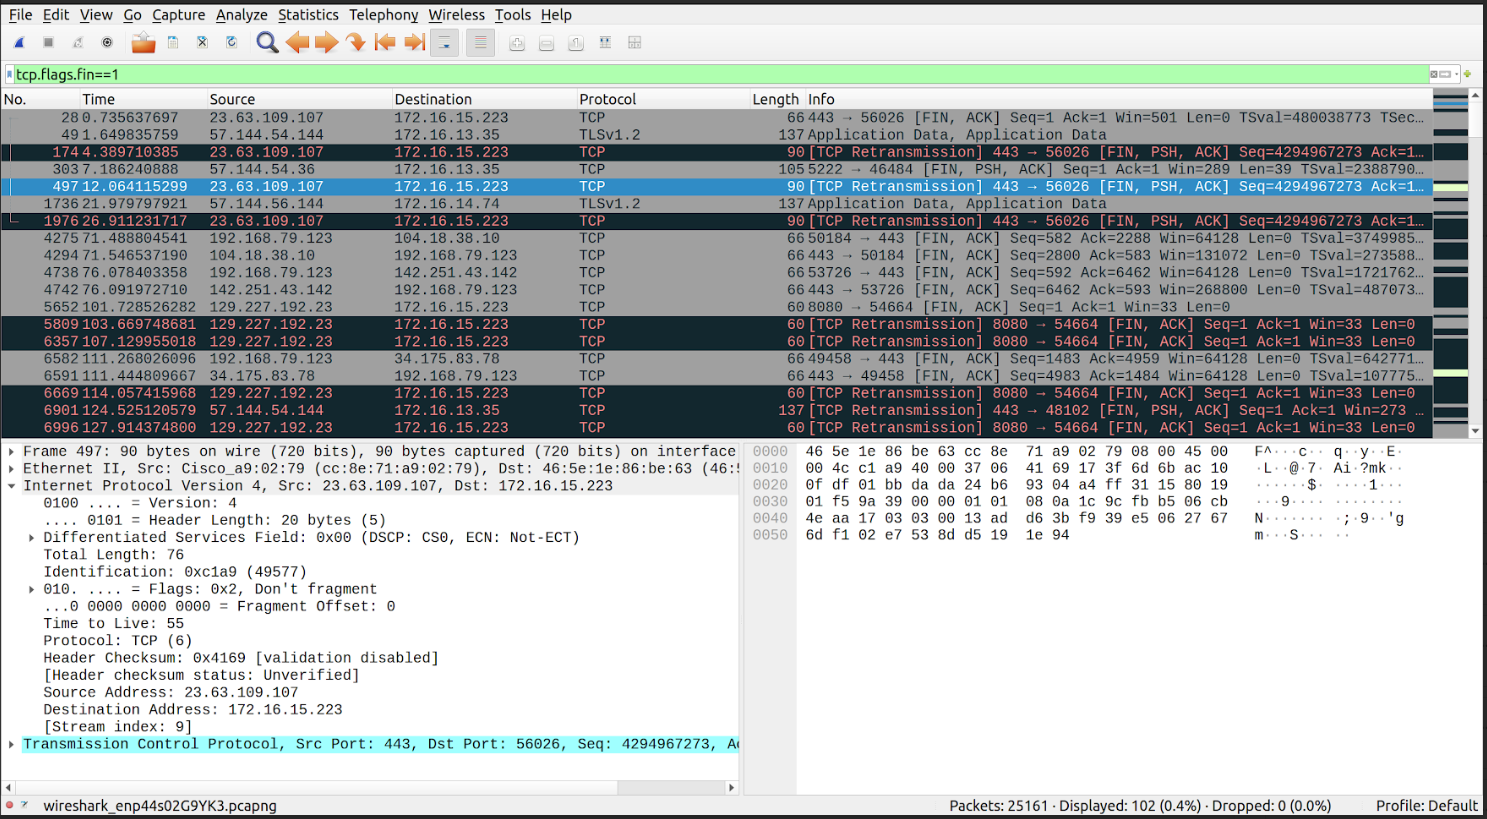
\includegraphics[width=0.8\textwidth]{assets/images/exp15/2.png}\\
\textbf{TCP FIN packet} (\texttt{tcp.flags.fin == 1})

\newpage
\textbf{B. Protocol-Based Packet Filtering}\\[0.3cm]
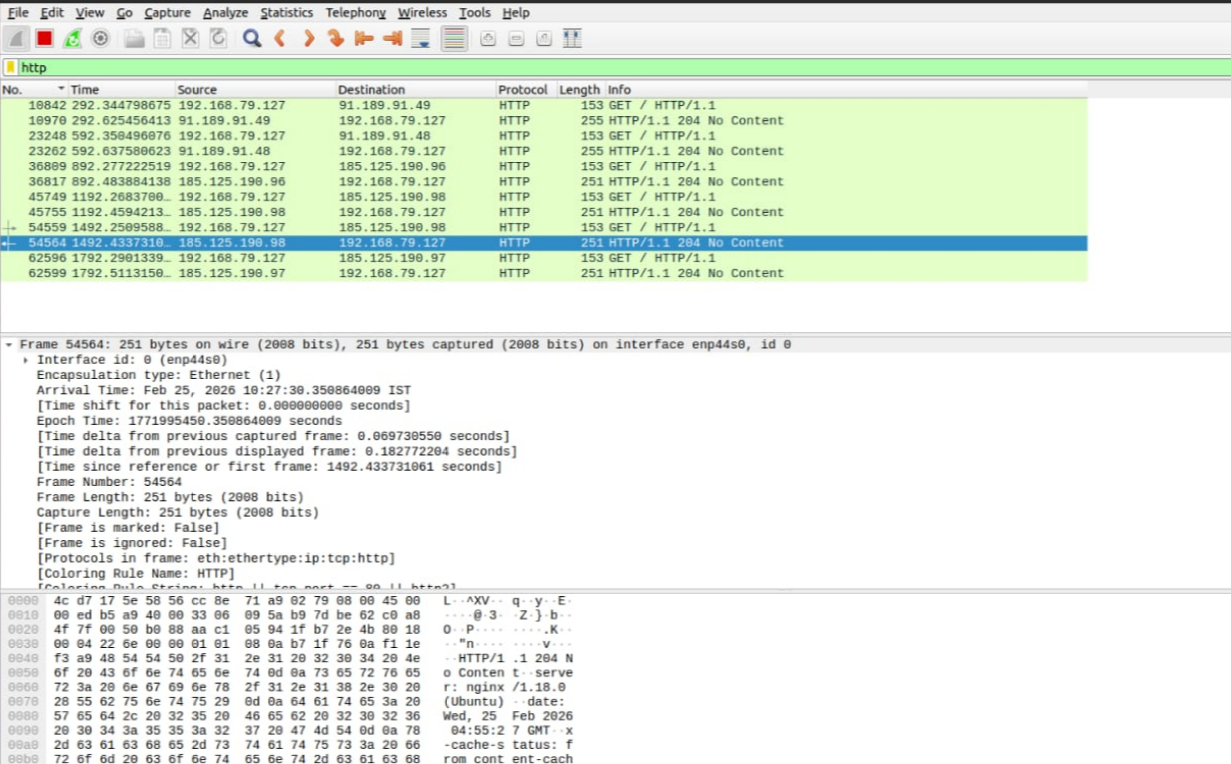
\includegraphics[width=0.8\textwidth]{assets/images/exp15/16.png}\\
\textbf{HTTP packets} (\texttt{http})\\[0.4cm]
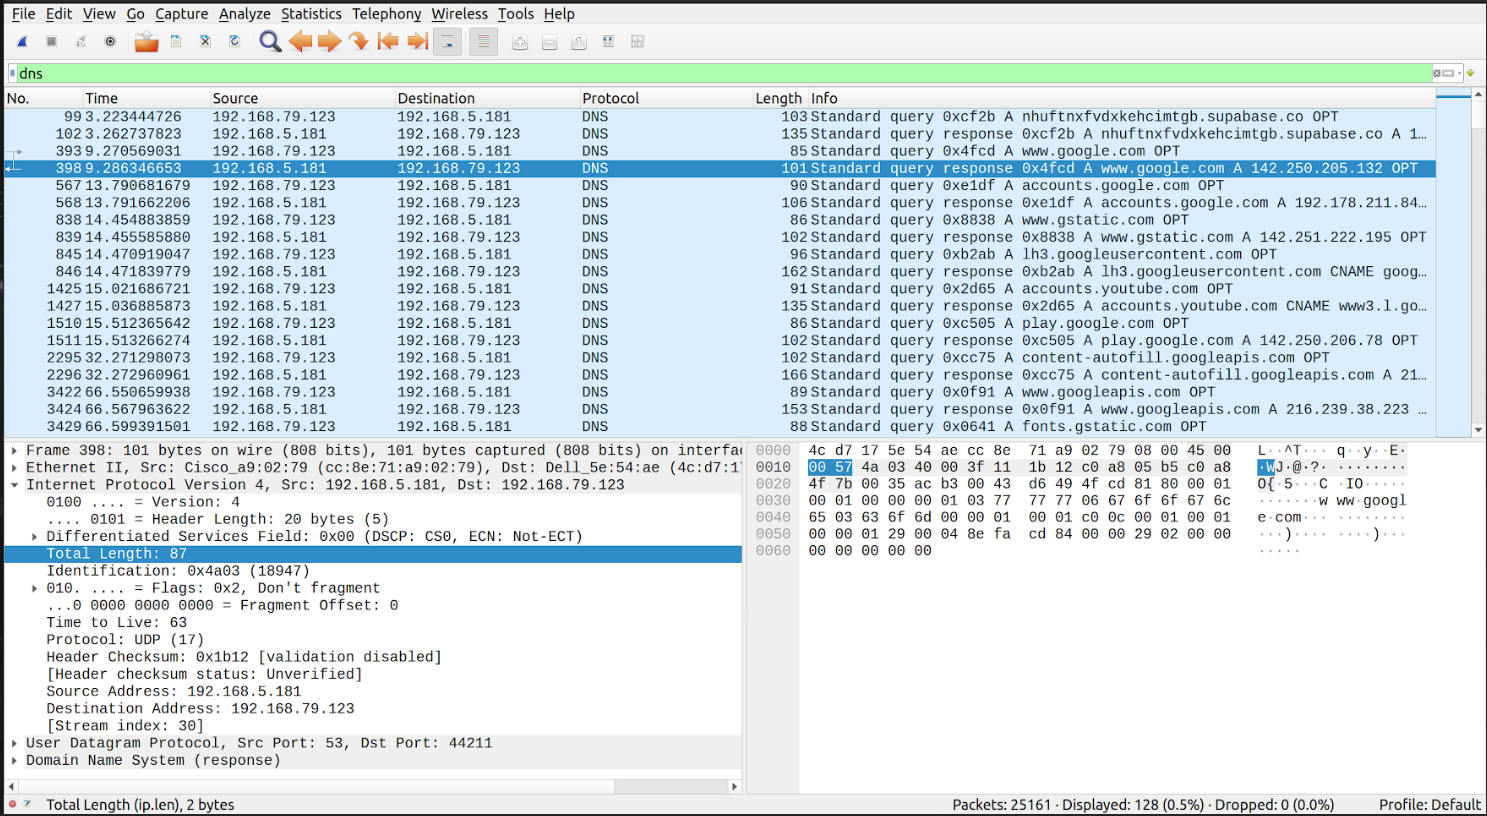
\includegraphics[width=0.8\textwidth]{assets/images/exp15/10.png}\\
\textbf{DNS packets} (\texttt{dns})\\[0.4cm]
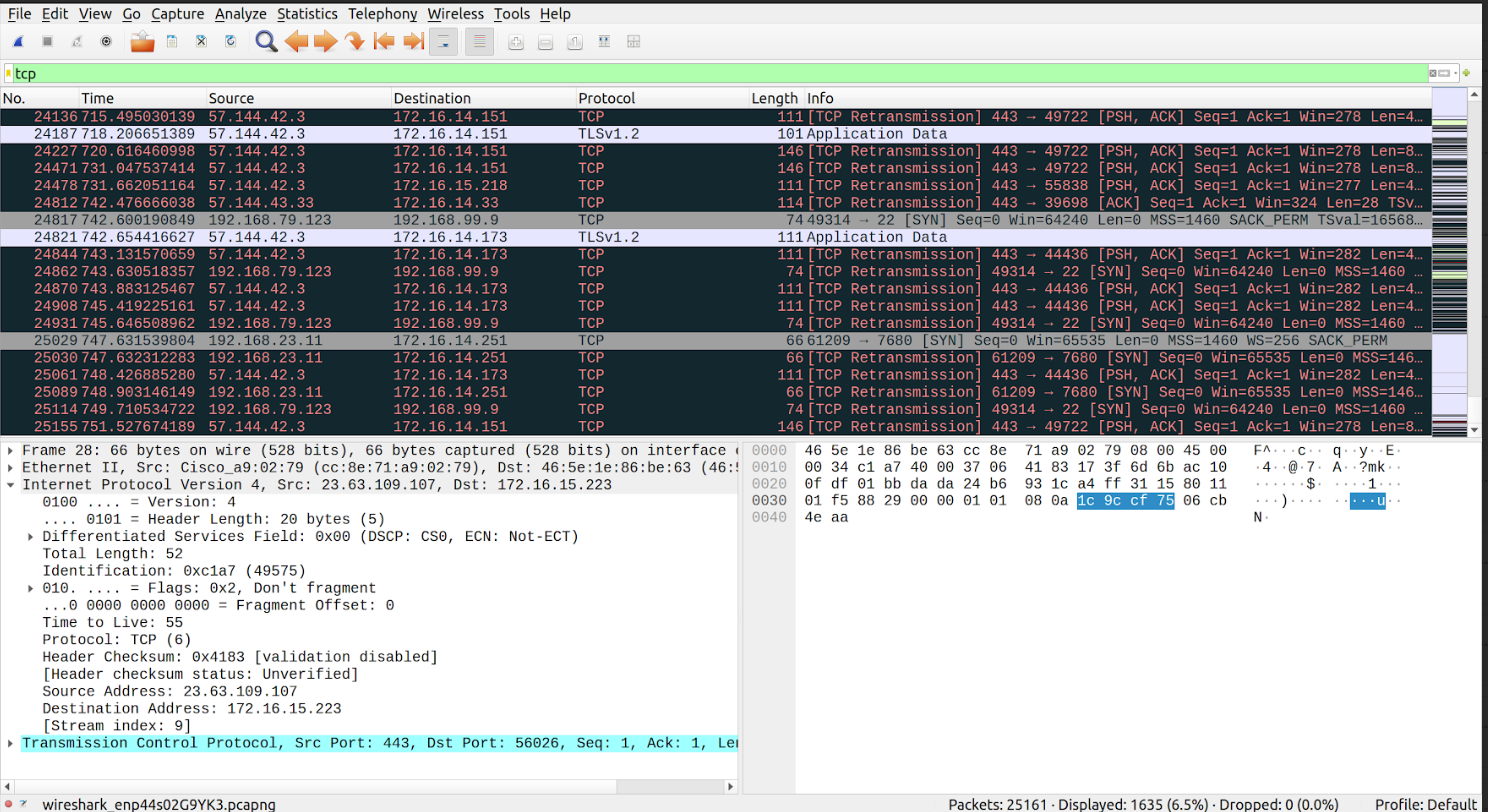
\includegraphics[width=0.8\textwidth]{assets/images/exp15/3.png}\\
\textbf{TCP packets} (\texttt{tcp})\\[0.4cm]
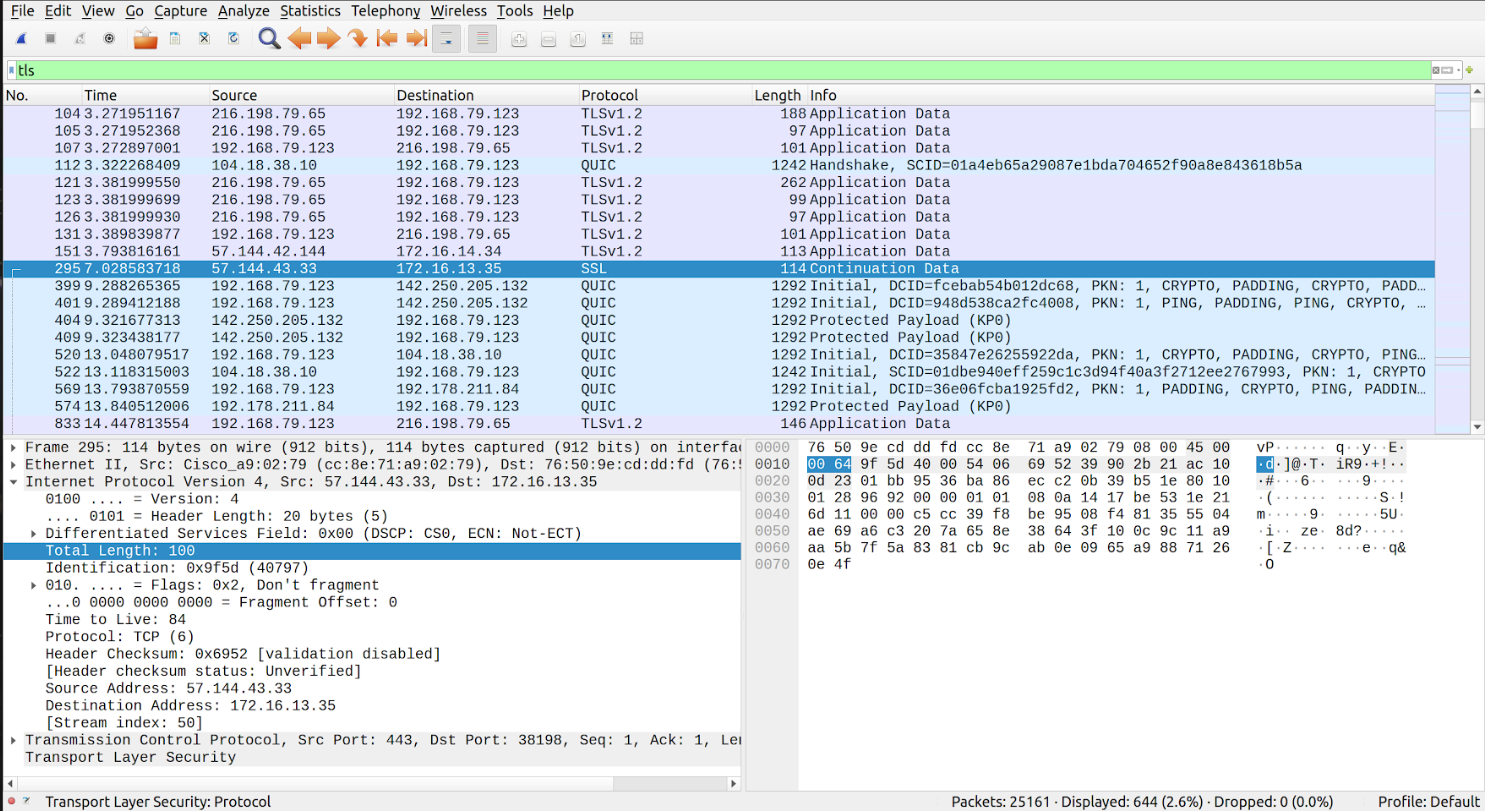
\includegraphics[width=0.8\textwidth]{assets/images/exp15/8.png}\\
\textbf{TLS packets} (\texttt{tls})\\[0.4cm]
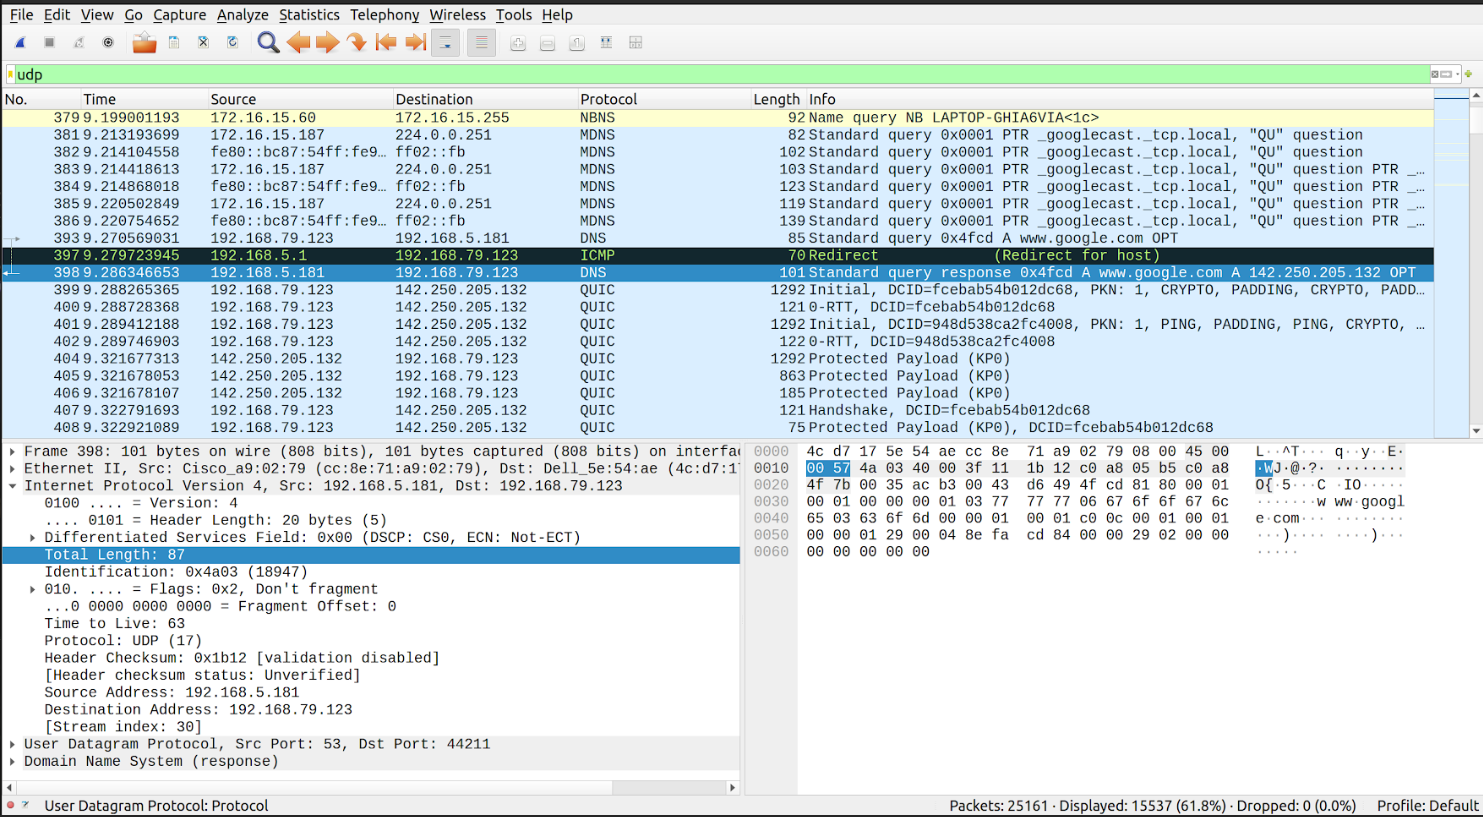
\includegraphics[width=0.8\textwidth]{assets/images/exp15/9.png}\\
\textbf{UDP packets} (\texttt{udp})

\newpage
\textbf{C. Statistics and Conversation Analysis}\\[0.3cm]
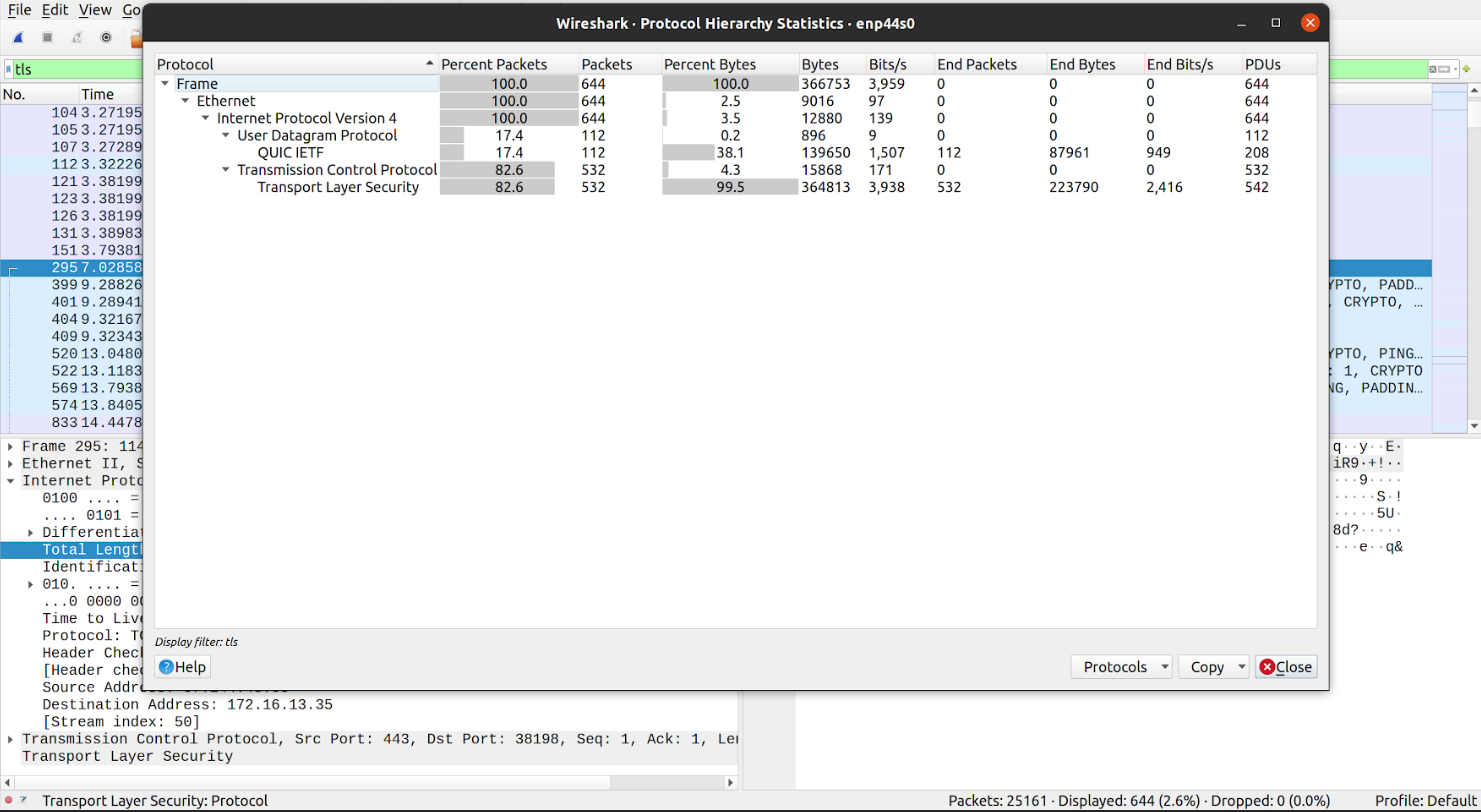
\includegraphics[width=0.8\textwidth]{assets/images/exp15/7.png}\\
\textbf{Protocol Hierarchy Statistics}\\[0.4cm]
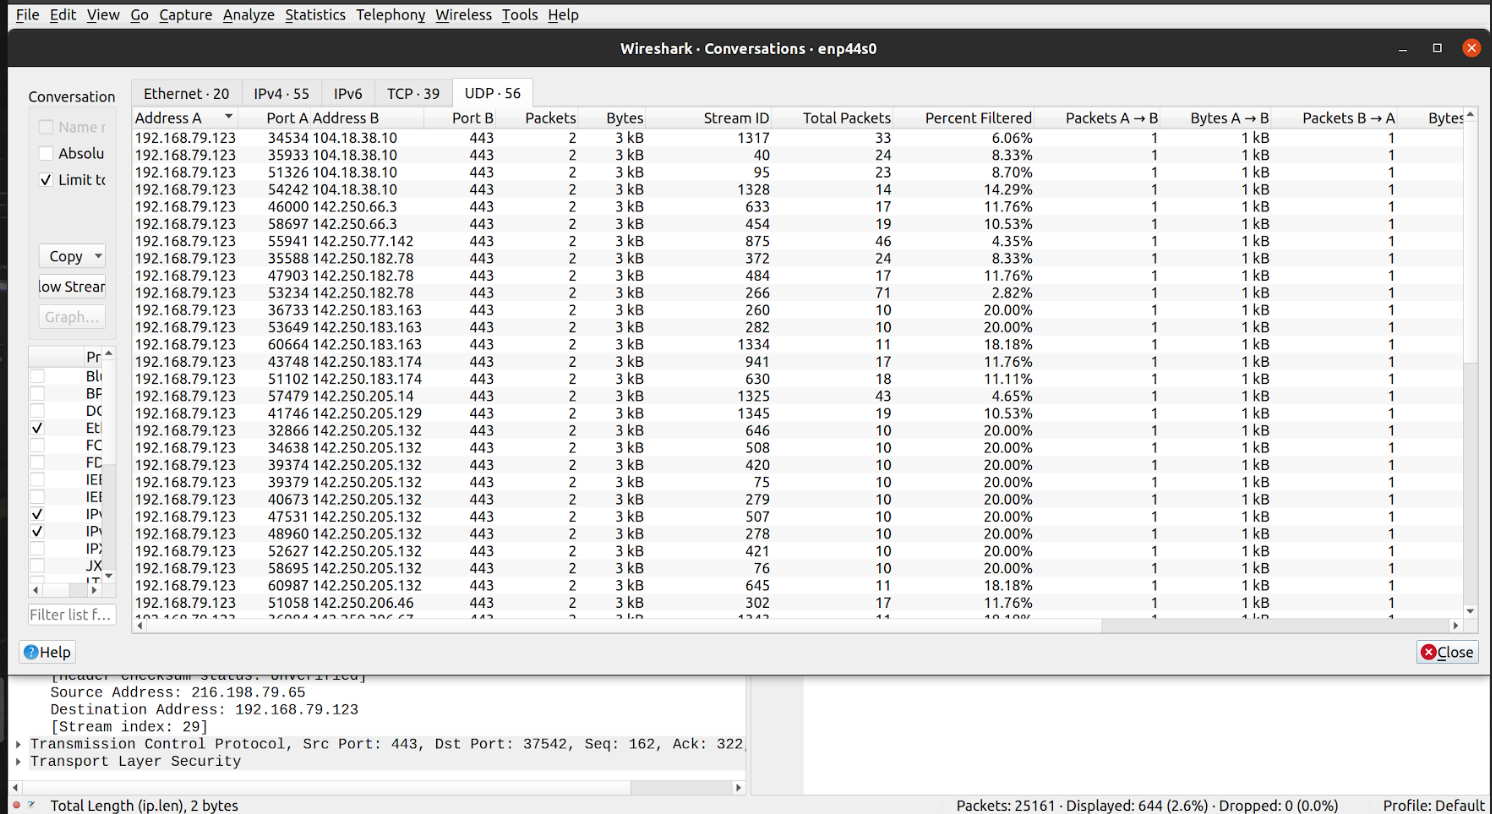
\includegraphics[width=0.8\textwidth]{assets/images/exp15/11.png}\\
\textbf{Conversations - UDP}\\[0.4cm]
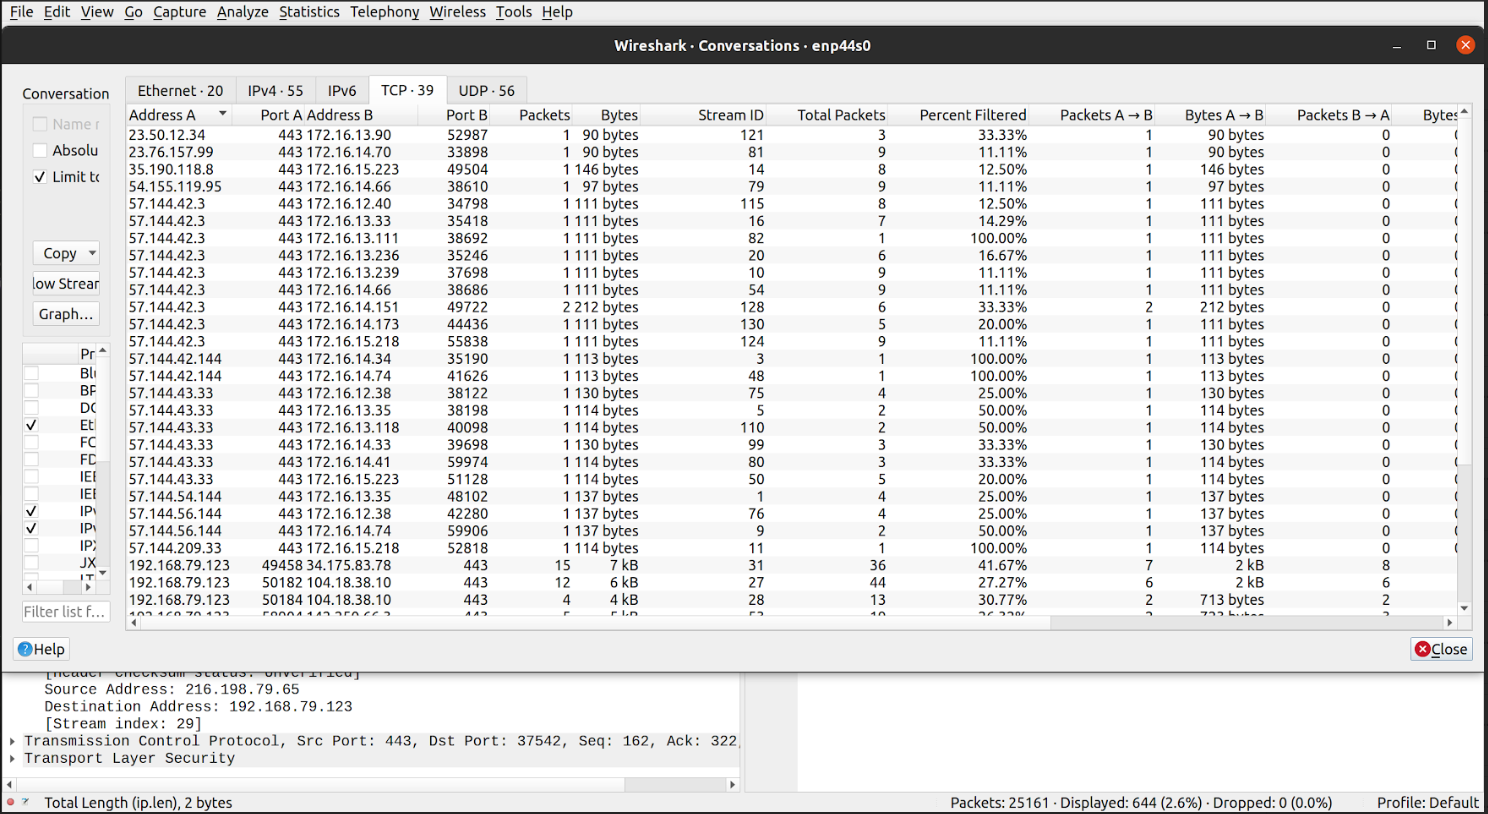
\includegraphics[width=0.8\textwidth]{assets/images/exp15/12.png}\\
\textbf{Conversations - TCP}\\[0.4cm]
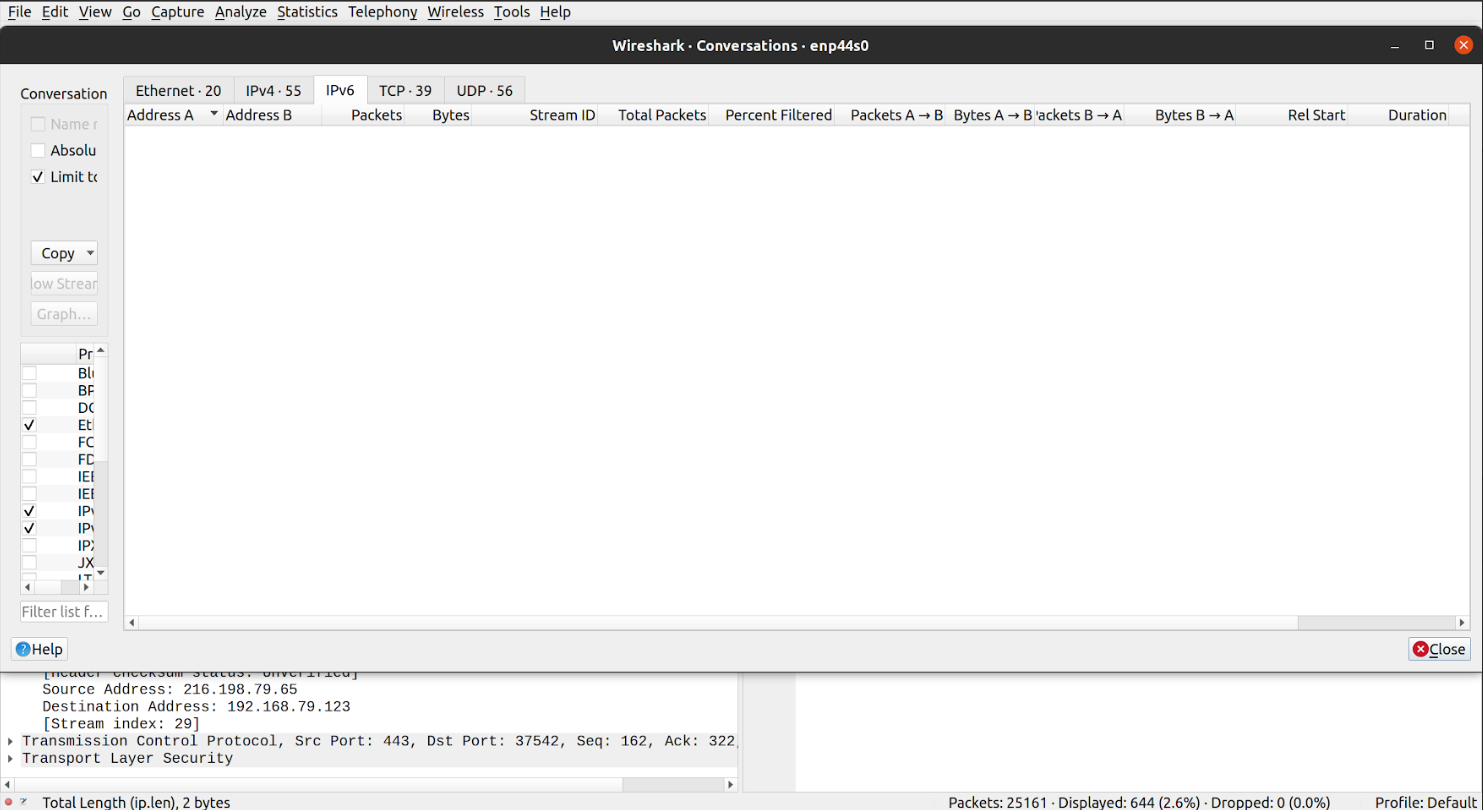
\includegraphics[width=0.8\textwidth]{assets/images/exp15/13.png}\\
\textbf{Conversations - IPv6}\\[0.4cm]
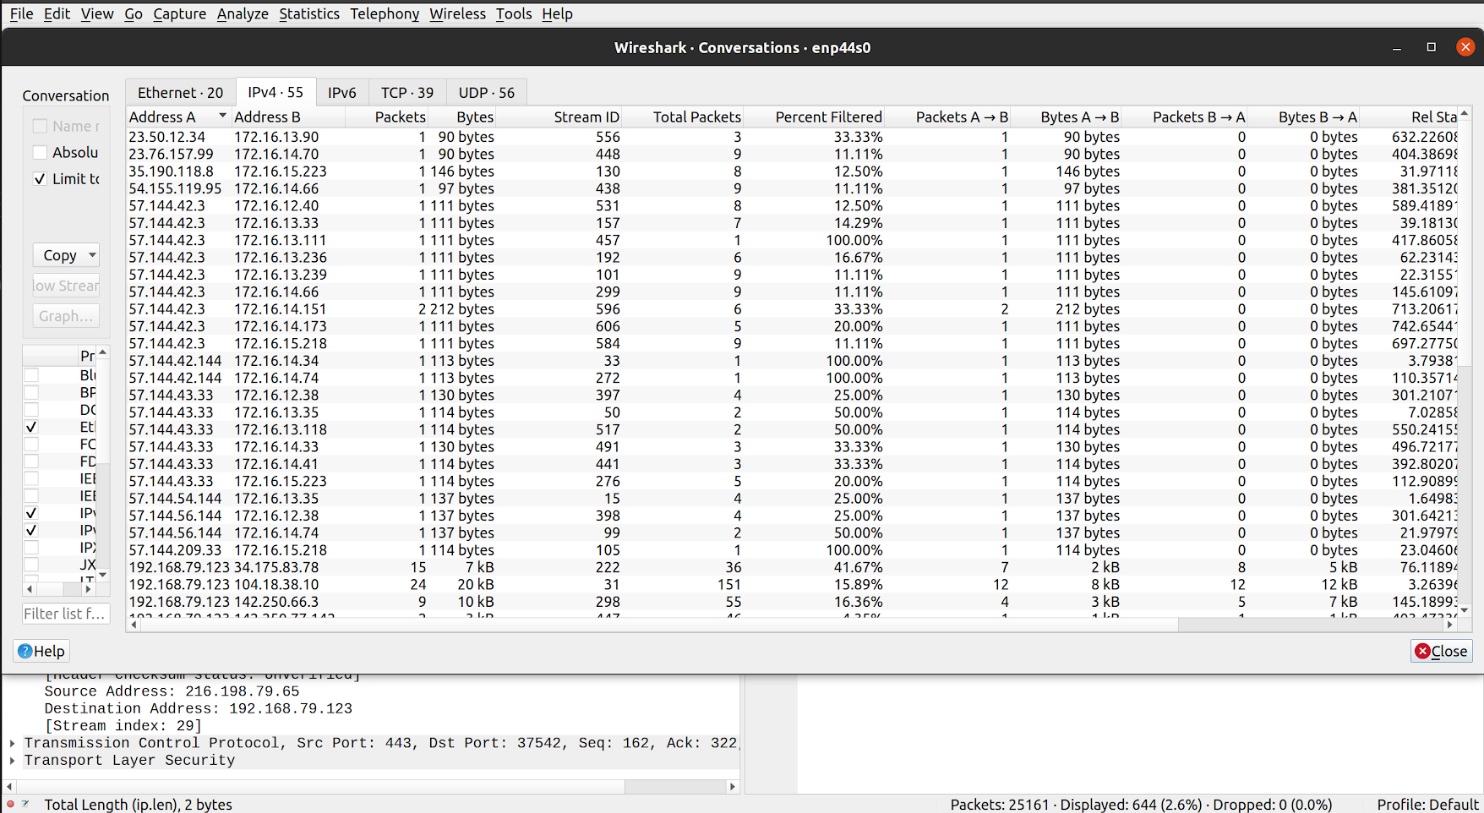
\includegraphics[width=0.8\textwidth]{assets/images/exp15/14.png}\\
\textbf{Conversations - IPv4}\\[0.4cm]
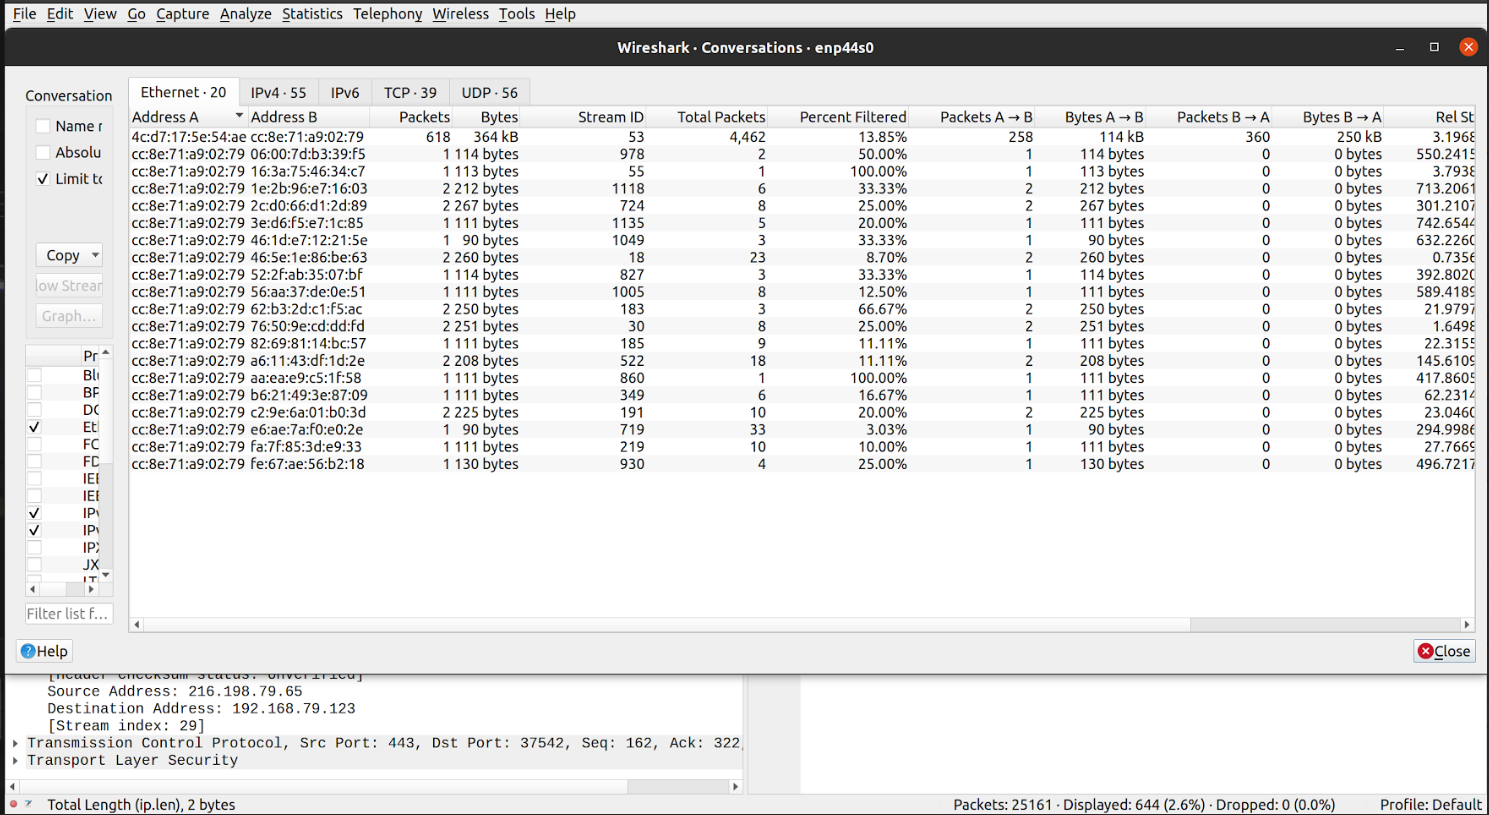
\includegraphics[width=0.8\textwidth]{assets/images/exp15/15.png}\\
\textbf{Conversations - Ethernet}

\newpage
\textbf{D. Graphical Visualization}\\[0.3cm]
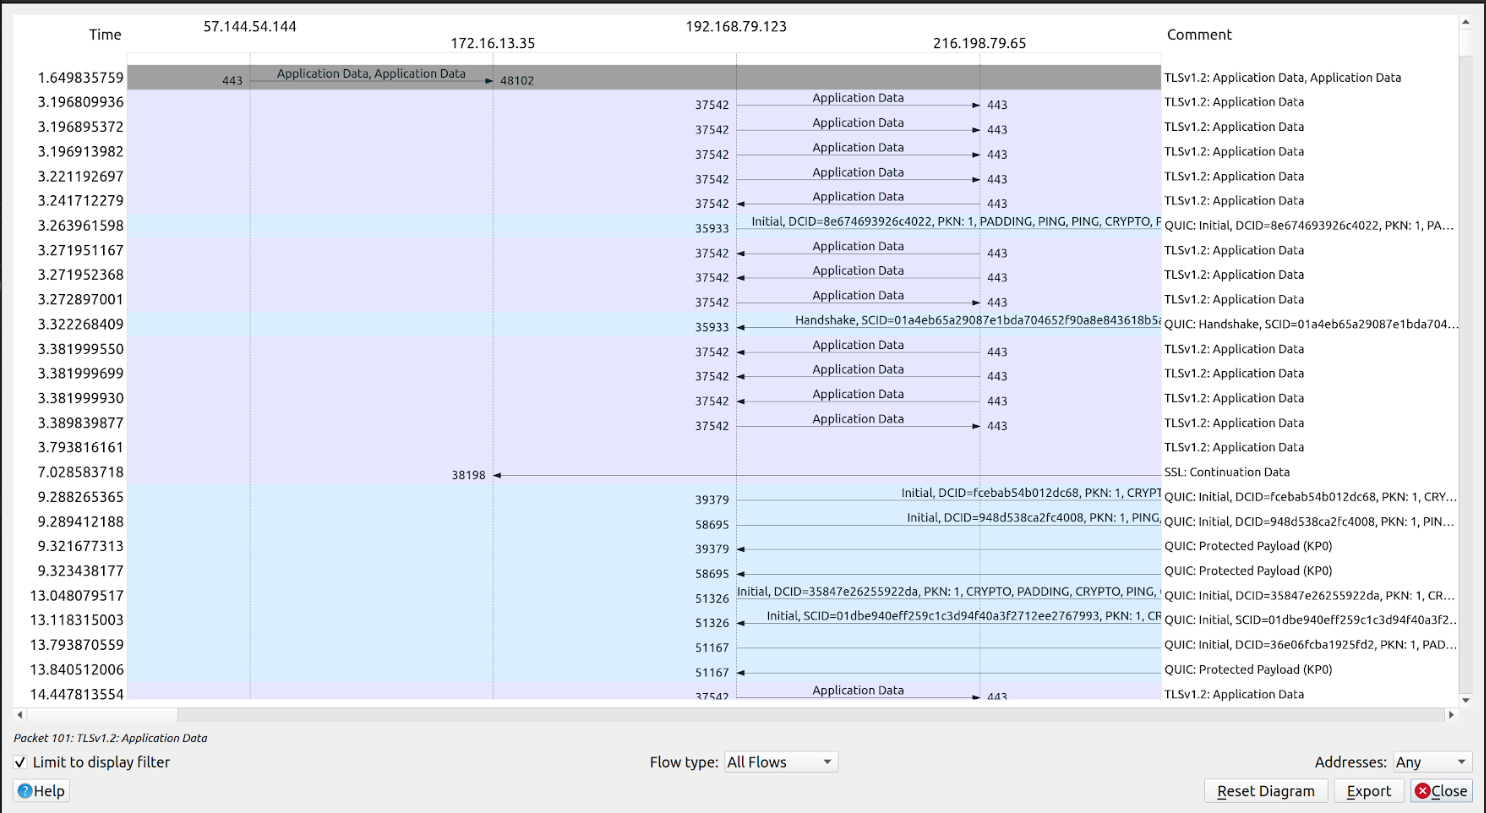
\includegraphics[width=0.8\textwidth]{assets/images/exp15/6.png}\\
\textbf{Flow Graph}\\[0.4cm]
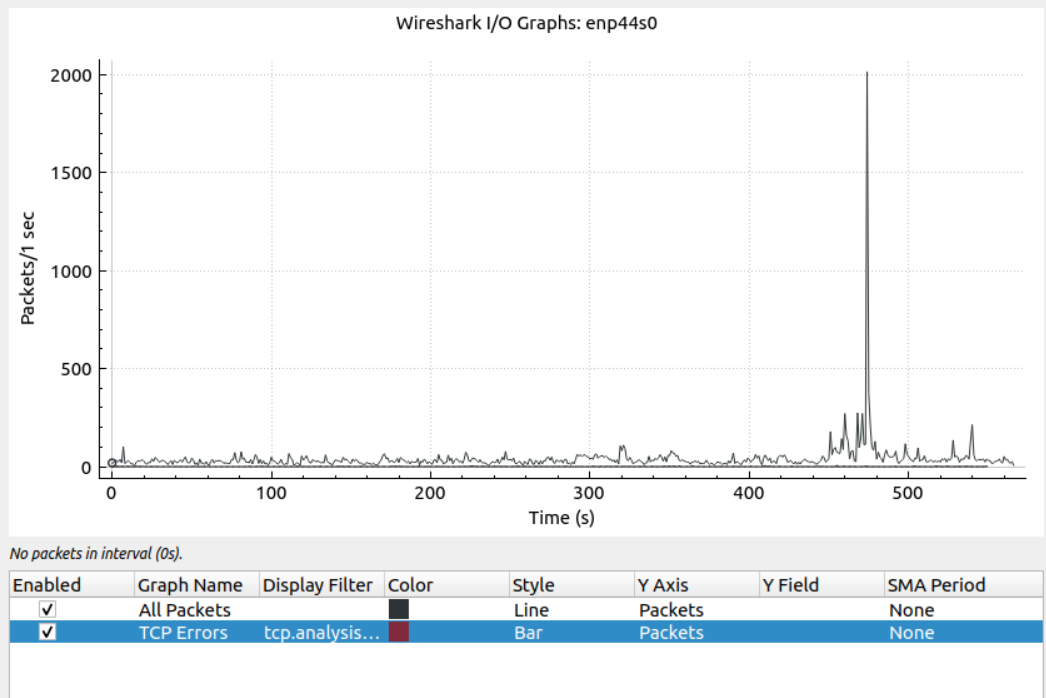
\includegraphics[width=0.8\textwidth]{assets/images/exp15/17.png}\\
\textbf{I/O Graph}\\[0.4cm]
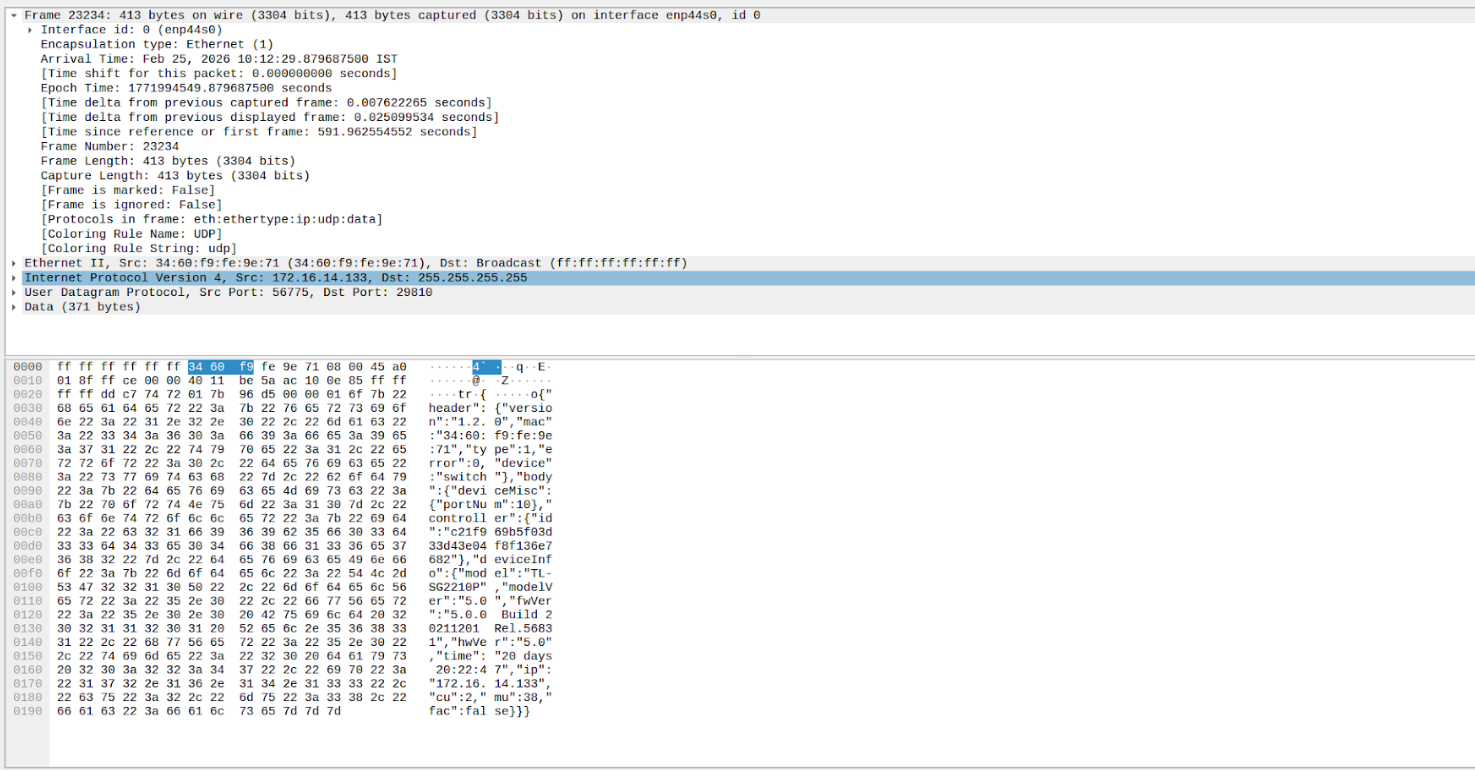
\includegraphics[width=0.8\textwidth]{assets/images/exp15/18.png}\\
\textbf{Packet Details Pane}
\end{center}
\subsection{Result}
TCP handshaking and network services were successfully analyzed using Wireshark display filters.

%%%%%%%%%%%%%%%%%%%%%%%%%%%%%%%%%



\experiment{NS2 Network Services Simulation}{28/02/2026}

\subsection{Aim}
To design and simulate a simple network topology in NS2 and configure TELNET, FTP, and DNS services using TCP and UDP.

\subsection{Theory}
NS2 (Network Simulator Version 2) is an open-source, event-driven simulator widely used for network research. It supports the simulation of both wired and wireless networks. NS2 uses Tcl scripts with OTcl object support to define and run simulations. The \texttt{nam} (Network Animator) tool provides graphical visualization of topology and packet flow.

\textbf{TELNET:}
\begin{itemize}
    \item Remote-login protocol
    \item Uses TCP (port 23)
    \item Interactive communication (small packets)
    \item Reliable and ordered delivery
\end{itemize}

\textbf{FTP:}
\begin{itemize}
    \item File Transfer Protocol
    \item Uses TCP
    \item Continuous bulk data transfer
    \item Reliable transmission
\end{itemize}

\textbf{DNS:}
\begin{itemize}
    \item Domain Name System
    \item Uses UDP
    \item Fast request--response communication
    \item Connectionless (no built-in reliability)
\end{itemize}

\subsection{Algorithm}
\begin{enumerate}
    \item Create a simulator instance and trace files.
    \item Create nodes: client, router, and server.
    \item Connect nodes using duplex links with bandwidth and delay.
    \item Configure TCP agents for TELNET and FTP.
    \item Configure UDP agent for DNS.
    \item Attach applications:
    \begin{itemize}
        \item Exponential traffic for TELNET
        \item FTP application for file transfer
        \item CBR traffic for DNS
    \end{itemize}
    \item Schedule start and stop times using \texttt{\$ns at}.
    \item Run simulation and visualize using NAM.
\end{enumerate}

% ---------------- TELNET ----------------
\subsection{Program for TELNET}
\begin{lstlisting}[language=tcl]
set ns [new Simulator]
set tf [open telnet.tr w]
$ns trace-all $tf
set nf [open telnet.nam w]
$ns namtrace-all $nf

set client [$ns node]
set router [$ns node]
set server [$ns node]

$ns duplex-link $client $router 10Mb 10ms DropTail
$ns duplex-link $router $server 10Mb 10ms DropTail

set tcp [new Agent/TCP]
$ns attach-agent $client $tcp
set sink [new Agent/TCPSink]
$ns attach-agent $server $sink
$ns connect $tcp $sink

set telnet [new Application/Traffic/Exponential]
$telnet attach-agent $tcp
$telnet set packetSize_ 200
$telnet set burst_time_ 0.5
$telnet set idle_time_ 0.5
$telnet set rate_ 100k

$ns at 1.0 "$telnet start"
$ns at 5.0 "finish"

proc finish {} {
    global ns tf nf
    $ns flush-trace
    close $tf
    close $nf
    exec nam telnet.nam &
    exit 0
}
$ns run
\end{lstlisting}
\subsubsection{Output}
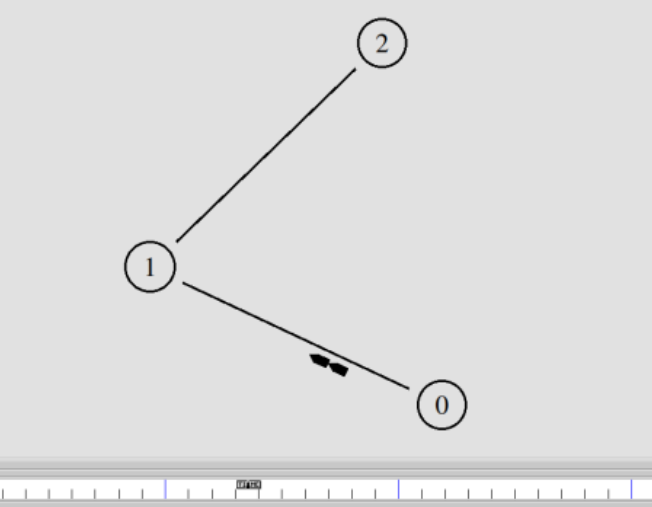
\includegraphics[width=0.60\textwidth]{assets/images/exp16/16a.png}
\subsubsection{TELNET Output Explanation}
\begin{itemize}
    \item Before 1 s: no traffic (idle network)
    \item Around 1 s: TCP three-way handshake occurs (SYN, SYN-ACK, ACK)
    \item After connection: small burst packets are transmitted
    \item Traffic is intermittent (interactive nature)
\end{itemize}

% ---------------- FTP ----------------
\subsection{Program for FTP}
\begin{lstlisting}[language=tcl]
set ns [new Simulator]
set tf [open ftp.tr w]
$ns trace-all $tf
set nf [open ftp.nam w]
$ns namtrace-all $nf

set client [$ns node]
set router [$ns node]
set server [$ns node]

$ns duplex-link $client $router 10Mb 10ms DropTail
$ns duplex-link $router $server 10Mb 10ms DropTail

set tcp [new Agent/TCP]
$ns attach-agent $client $tcp
set sink [new Agent/TCPSink]
$ns attach-agent $server $sink
$ns connect $tcp $sink

set ftp [new Application/FTP]
$ftp attach-agent $tcp

$ns at 1.0 "$ftp start"
$ns at 5.0 "finish"

proc finish {} {
    global ns tf nf
    $ns flush-trace
    close $tf
    close $nf
    exec nam ftp.nam &
    exit 0
}
$ns run
\end{lstlisting}
\subsubsection{Output}
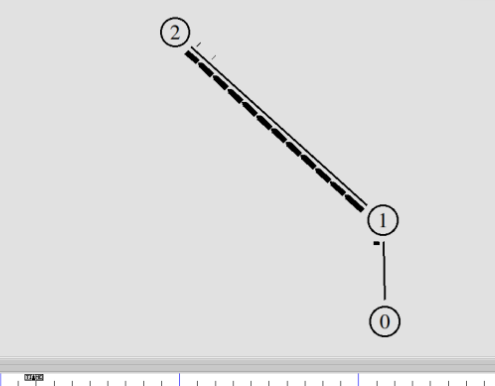
\includegraphics[width=0.60\textwidth]{assets/images/exp16/16b.png}
\subsubsection{FTP Output Explanation}
\begin{itemize}
    \item Continuous packet transmission after 1 s
    \item TCP handshake occurs first
    \item Dense traffic flow (bulk data transfer)
    \item ACK packets ensure reliability
\end{itemize}

% ---------------- DNS ----------------
\subsection{Program for DNS}
\begin{lstlisting}[language=tcl]
set ns [new Simulator]
set tf [open dns.tr w]
$ns trace-all $tf
set nf [open dns.nam w]
$ns namtrace-all $nf

set client [$ns node]
set router [$ns node]
set server [$ns node]

$ns duplex-link $client $router 10Mb 10ms DropTail
$ns duplex-link $router $server 10Mb 10ms DropTail

set udp [new Agent/UDP]
$ns attach-agent $client $udp
set null [new Agent/Null]
$ns attach-agent $server $null
$ns connect $udp $null

set cbr [new Application/Traffic/CBR]
$cbr attach-agent $udp
$cbr set packetSize_ 512
$cbr set interval_ 0.2

$ns at 1.0 "$cbr start"
$ns at 5.0 "finish"

proc finish {} {
    global ns tf nf
    $ns flush-trace
    close $tf
    close $nf
    exec nam dns.nam &
    exit 0
}
$ns run
\end{lstlisting}
\subsubsection{Output}
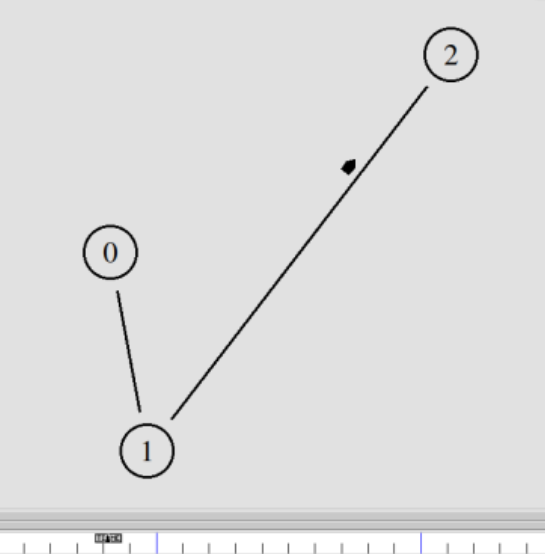
\includegraphics[width=0.60\textwidth]{assets/images/exp16/16c.png}
\subsubsection{DNS Output Explanation}
\begin{itemize}
    \item Uses UDP (no acknowledgements)
    \item Small request--response packets
    \item Faster communication compared to TCP
    \item No congestion control or reliability
\end{itemize}



\subsection{Result}
TELNET, FTP, and DNS services were successfully simulated in the NS2 environment using TCP and UDP. The behavior of interactive, bulk, and request--response traffic was observed and analyzed using NAM visualization.

%%%%%%%%%%%%%%%%%%%%%%%%%%%%%%%%%



\experiment{TCP Reno Analysis in NS2}{28/02/2026}

\subsection{Aim}
To analyze TCP Reno congestion window dynamics in a two-node NS2 simulation.

\subsection{Theory}
TCP Reno is a widely used TCP congestion-control algorithm that extends TCP Tahoe by introducing Fast Recovery. When a Reno sender receives three duplicate acknowledgments, it infers packet loss while assuming that the network can still deliver data. Instead of reducing the congestion window to 1 (as in Tahoe slow start), Reno halves the window and enters fast recovery, thereby improving throughput.

\subsection{Algorithm}
\begin{enumerate}
    \item Initialize the \texttt{Simulator} object and trace files.
    \item Build a basic two-node layout using \texttt{duplex-link}.
    \item Spawn \texttt{Agent/TCP/Reno} and attach it to the source. Create a \texttt{TCPSink} on the destination node.
    \item Define a Tcl procedure named \texttt{record} that recursively logs the \texttt{cwnd\_} (congestion window) property of the TCP agent every 0.1 seconds.
    \item Execute FTP data transfer over the Reno agent and trace the window adjustment behaviors (Slow Start, Congestion Avoidance, Fast Retransmit).
\end{enumerate}

\subsection{Program}
\begin{lstlisting}[language=tcl]
# Create simulator
set ns [new Simulator]
# Trace files
set tracefile [open out.tr w]
$ns trace-all $tracefile
set namfile [open out.nam w]
$ns namtrace-all $namfile
# Create nodes
set n0 [$ns node]
set n1 [$ns node]
# Create duplex link (wired)
$ns duplex-link $n0 $n1 10Mb 10ms DropTail
$ns queue-limit $n0 $n1 50

# TCP Reno
set tcp [new Agent/TCP/Reno]
$tcp set class_ 2
$ns attach-agent $n0 $tcp
# TCP Sink
set sink [new Agent/TCPSink]
$ns attach-agent $n1 $sink
# Connect
$ns connect $tcp $sink
# FTP
set ftp [new Application/FTP]
$ftp attach-agent $tcp
# Start/Stop FTP
$ns at 0.5 "$ftp start"
$ns at 149.0 "$ftp stop"
# Record CWND
set cwndfile [open cwnd.tr w]
proc record {} {
global tcp cwndfile ns
set time [$ns now]
set cwnd [$tcp set cwnd_]
puts $cwndfile "$time $cwnd"
$ns at [expr $time + 0.1] "record"
}
$ns at 0.1 "record"
# Finish
proc finish {} {
global ns tracefile namfile cwndfile
$ns flush-trace
close $tracefile
close $namfile
close $cwndfile
exec nam out.nam &
exit 0
}
$ns at 150.0 "finish"
$ns run
\end{lstlisting}

\subsection{Output}
\noindent\textbf{Program Execution}

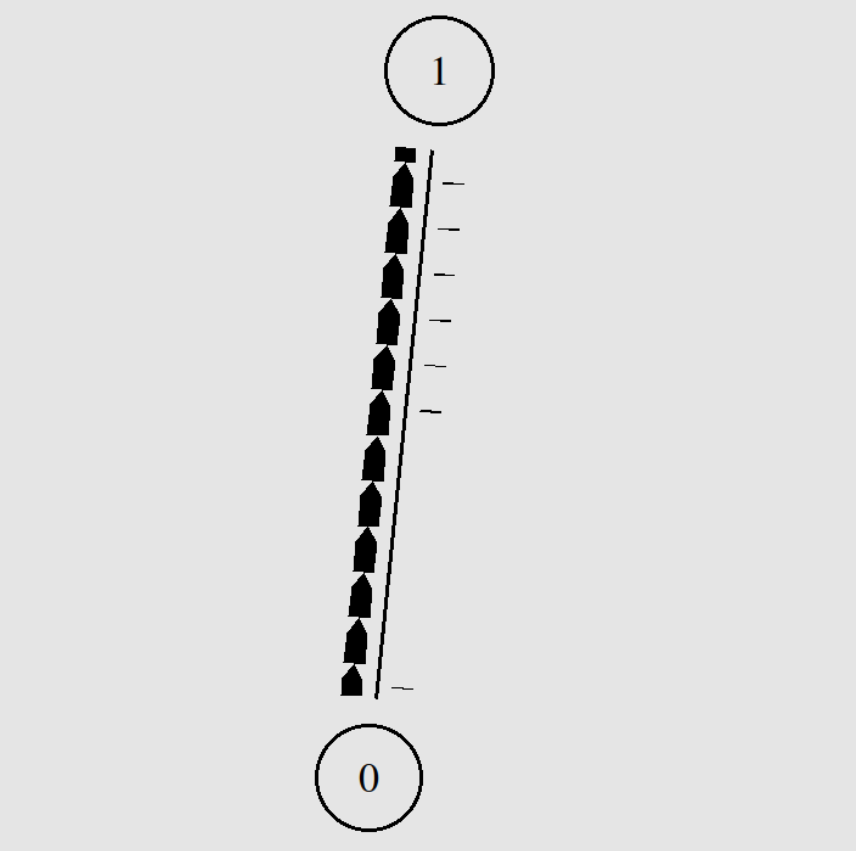
\includegraphics[width=0.6\textwidth]{assets/images/exp17/17.0.png}
\begin{verbatim}
ns tcp_reno.tcl
Wait until terminal returns.
Then check:

cat cwnd.tr | head
0.10000000000000001 1
0.20000000000000001 1
0.30000000000000004 1
0.40000000000000002 1
0.5 1
0.59999999999999998 16
0.69999999999999996 24.0038
0.79999999999999993 27.6826
0.89999999999999991 30.9263
0.99999999999999989 33.8604

gnuplot
Then:
plot "cwnd.tr" with lines
\end{verbatim}

\noindent\textbf{Congestion Window Plot}

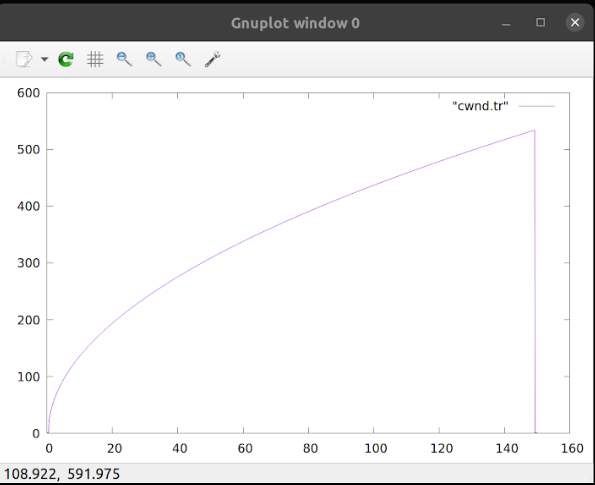
\includegraphics[width=0.6\textwidth]{assets/images/exp17/17.2.png}

\subsection{Result}
TCP Reno congestion-window dynamics were successfully traced and written to a trace file for plotting and analysis.

%%%%%%%%%%%%%%%%%%%%%%%%%%%%%%%%%



\experiment{Ping over Star Topology in NS2}{28/02/2026}

\subsection{Aim}
To simulate ping transmission over a star topology and observe packet behavior across multiple nodes in NS2.

\subsection{Theory}
A star topology consists of one central node (hub/switch) connected to all peripheral nodes. In NS2, the \texttt{Agent/Ping} module can be used to simulate ICMP Echo Request and Echo Reply communication. By attaching ping agents to peripheral nodes and routing traffic through the central node, the simulator can measure Round-Trip Time (RTT).

\subsection{Algorithm}
\begin{enumerate}
    \item Construct a \texttt{Simulator} object.
    \item Declare one central hub node. Use a \texttt{for} loop to instantiate multiple peripheral nodes, linking them to the hub via \texttt{duplex-link} to form a star topology.
    \item Attach \texttt{Agent/Ping} modules to the peripheral nodes.
    \item Intercept ping replies by overriding the \texttt{Agent/Ping instproc recv} method. Extract and print the Round-Trip Time (RTT).
    \item Use \texttt{\$ns at} to schedule ping bursts between nodes.
\end{enumerate}

\subsection{Program}
\begin{lstlisting}[language=tcl]
# Create simulator
set ns [new Simulator]
# Trace files
set tracefile [open out.tr w]
$ns trace-all $tracefile
set namfile [open out.nam w]
$ns namtrace-all $namfile
# Number of nodes (1 center + 6 leaf nodes)
set n 7
# Create nodes
for {set i 0} {$i < $n} {incr i} {
set node($i) [$ns node]
}
# Star topology (very low bandwidth + small queue)
for {set i 1} {$i < $n} {incr i} {
$ns duplex-link $node(0) $node($i) 0.2Mb 10ms DropTail
$ns queue-limit $node(0) $node($i) 2
}
# Central receiver

set null [new Agent/Null]
$ns attach-agent $node(0) $null
# Heavy traffic from all leaf nodes
for {set i 1} {$i < $n} {incr i} {
set udp($i) [new Agent/UDP]
$ns attach-agent $node($i) $udp($i)
$ns connect $udp($i) $null
set cbr($i) [new Application/Traffic/CBR]
$cbr($i) set packetSize_ 1000
$cbr($i) set interval_ 0.001
$cbr($i) attach-agent $udp($i)
$ns at 0.2 "$cbr($i) start"
$ns at 4.5 "$cbr($i) stop"
}
# Finish
proc finish {} {
global ns tracefile namfile
$ns flush-trace
close $tracefile
close $namfile
exec nam out.nam &
exit 0
}
$ns at 5.0 "finish"
$ns run
\end{lstlisting}

\subsection{Output}
\noindent\textbf{Simulation Output}


\includegraphics[width=0.6\textwidth]{assets/images/exp18/18.png}
\begin{verbatim}
grep "^d" out.tr | wc -l
24864 packets dropped
\end{verbatim}

\subsection{Result}
The star-topology ping simulation and Round-Trip Time (RTT) detection were successfully executed.

%%%%%%%%%%%%%%%%%%%%%%%%%%%%%%%%%



\experiment{Distance Vector Routing in NS2}{28/02/2026}

\subsection{Aim}
To simulate rerouting behavior during link failure using dynamic distance-vector routing in NS2.

\subsection{Theory}
Dynamic routing protocols automatically adjust routes based on topology changes. In NS2, distance-vector behavior can be studied using protocols such as DSDV. When route conditions change, the protocol updates forwarding paths and reroutes traffic through available alternate paths.

\subsection{Algorithm}
\begin{enumerate}
    \item Initialize the \texttt{Simulator} and configure dynamic routing.
    \item Create wireless nodes and configure DSDV as the ad hoc routing protocol.
    \item Attach UDP and Null agents, then generate CBR traffic from source to destination.
    \item Start and stop traffic at scheduled times using \texttt{\$ns at} events.
    \item Run the simulation, observe routing behavior in NAM, and analyze trace output.
\end{enumerate}

\subsection{Program}
\begin{lstlisting}[language=tcl]
# DSDV Routing Protocol in NS2
# Create Simulator
set ns [new Simulator]
# Open Trace File
set tracefile [open out.tr w]
$ns trace-all $tracefile
# Open NAM File
set namfile [open out.nam w]
$ns namtrace-all-wireless $namfile 500 500
# Define Topography
set topo [new Topography]
$topo load_flatgrid 500 500
# Number of nodes
set val(nn) 4
create-god $val(nn)
# Configure Nodes (DSDV Routing)
$ns node-config -adhocRouting DSDV \
-llType LL \
-macType Mac/802_11 \
-ifqType Queue/DropTail/PriQueue \
-ifqLen 50 \
-antType Antenna/OmniAntenna \
-propType Propagation/TwoRayGround \
-phyType Phy/WirelessPhy \
-channelType Channel/WirelessChannel \
-topoInstance $topo \
-agentTrace ON \
-routerTrace ON \
-macTrace OFF
# Create Nodes
set n0 [$ns node]

set n1 [$ns node]
set n2 [$ns node]
set n3 [$ns node]
# Set Positions
$n0 set X_ 100; $n0 set Y_ 100; $n0 set Z_ 0
$n1 set X_ 300; $n1 set Y_ 100; $n1 set Z_ 0
$n2 set X_ 100; $n2 set Y_ 300; $n2 set Z_ 0
$n3 set X_ 300; $n3 set Y_ 300; $n3 set Z_ 0
# Create UDP Agent
set udp [new Agent/UDP]
$ns attach-agent $n0 $udp
# Create Null Agent
set null [new Agent/Null]
$ns attach-agent $n3 $null
# Connect Agents
$ns connect $udp $null
# Create CBR Traffic
set cbr [new Application/Traffic/CBR]
$cbr set packetSize_ 512
$cbr set interval_ 0.2
$cbr attach-agent $udp
# Start and Stop Traffic
$ns at 1.0 "$cbr start"
$ns at 9.0 "$cbr stop"
# Finish Procedure
proc finish {} {
global ns tracefile namfile
$ns flush-trace
close $tracefile
close $namfile
exec nam out.nam &
exit 0
}
$ns at 10.0 "finish"
# Run Simulation
$ns run
\end{lstlisting}

\subsection{Output}
\begin{center}
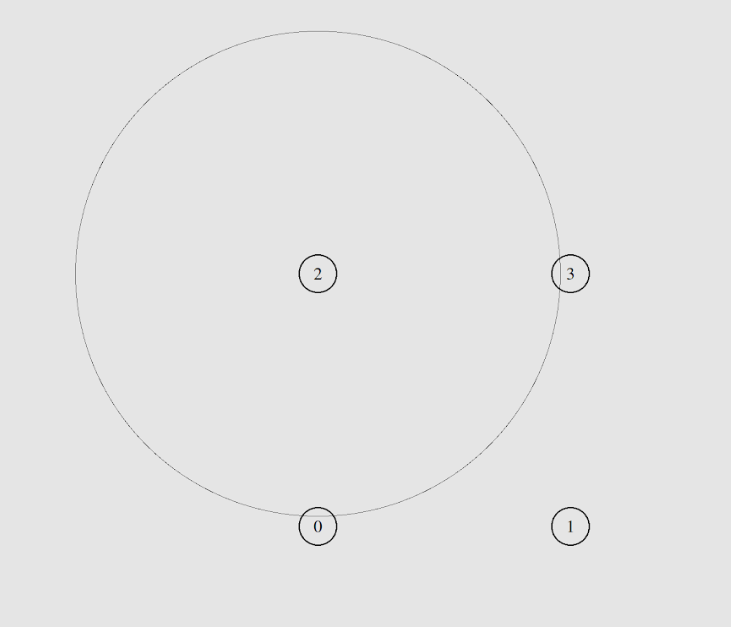
\includegraphics[width=0.6\textwidth]{assets/images/exp19/19.png}
\\[0.2cm]
\textbf{Distance-Vector Routing Simulation Output}
\end{center}

\subsection{Result}
Dynamic routing behavior was successfully demonstrated in NS2 using a distance-vector-based protocol (DSDV).

%%%%%%%%%%%%%%%%%%%%%%%%%%%%%%%%%

\end{document}
